\documentclass[11pt, a4paper]{report} % add draft if needed

\usepackage[english]{babel}
\usepackage[T1]{fontenc}
\usepackage[utf8]{inputenc}
\usepackage{mathtools}
\usepackage{amsfonts}
\usepackage{listings}
\usepackage[a4paper]{geometry}
\usepackage{longtable}
\usepackage{booktabs}
\usepackage[parfill]{parskip}
\usepackage{hyperref}
\usepackage{lipsum}
\usepackage[toc,page]{appendix}
\usepackage{lastpage}
\usepackage{fancyhdr}
\usepackage[explicit]{titlesec}
\usepackage[style=alphabetic]{biblatex}
\usepackage{color}
\usepackage{amsthm}
\usepackage{todo}
\usepackage{tikz}
\usepackage{subcaption}
\usepackage{caption}
\usepackage{chemfig}
\usepackage{cleveref}
\usepackage{multicol}
\usepackage[newfloat]{minted}
\usepackage{mdframed}

\interfootnotelinepenalty=3000

\setcounter{tocdepth}{1}

\providecommand{\tightlist}{%
  \setlength{\itemsep}{0pt}\setlength{\parskip}{0pt}}

\newenvironment{coded}{\captionsetup{type=listing}}{}

\setminted{linenos,frame=lines,framesep=2mm}
\setminted[text]{linenos=false}


%tikz extras
\usetikzlibrary{arrows, shapes, snakes, automata, backgrounds, positioning}

\tikzset{
    triple/.style args={[#1] in [#2] in [#3]}{
        #1,preaction={preaction={draw,#3},draw,#2}
    }
}

% math envirs
\theoremstyle{definition}
\newtheorem{defn}{Definition}
\newtheorem{obsv}{Observation}

\newenvironment{observation}
    {\begin{framed}\begin{obsv}}
    {\end{obsv}\end{framed}}

% Chapter title formatting
\definecolor{gray75}{gray}{0.75}
\newcommand{\hsp}{\hspace{20pt}}

\titleformat{\chapter}[display]{}{
}{-85pt}{\Huge\bfseries\centering\textcolor{gray75}{|}\hsp#1\hsp\textcolor{gray75}{|}\\\hspace{10pt}}

% Header and footer
\fancypagestyle{plain}{% plain style is used on chapter pages
  \fancyhf{}%
  \fancyfoot[C]{\thepage}% Page \thepage\ of \pageref*{LastPage}
  \renewcommand{\headrulewidth}{0pt}% Line at the header invisible
  %\renewcommand{\footrulewidth}{0.4pt}% Line at the footer visible
}

\pagestyle{fancy}
\fancypagestyle{MyStyle}{
    \fancyhf{}
    \fancyhead[L]{ \leftmark }
    \fancyhead[R]{ \today }
    \fancyfoot[C]{ \thepage } % chktex 2
    \renewcommand{\chaptermark}[1]{\markboth{\textsl{##1}}{}}
    \renewcommand{\headrulewidth}{0pt}
}

\newcommand{\blankpage}{
  \newpage
  \thispagestyle{empty}
  \mbox{}
  \newpage
}

% \definecolor{mygreen}{rgb}{0,0.6,0}
% \definecolor{mygray}{rgb}{0.5,0.5,0.5}
% \definecolor{mymauve}{rgb}{0.58,0,0.82}

% \lstset{ %
%   backgroundcolor=\color{white},   % choose the background color; you must add \usepackage{color} or \usepackage{xcolor}; should come as last argument
%   basicstyle=\footnotesize,        % the size of the fonts that are used for the code
%   breakatwhitespace=false,         % sets if automatic breaks should only happen at whitespace
%   breaklines=true,                 % sets automatic line breaking
%   captionpos=b,                    % sets the caption-position to bottom
%   commentstyle=\color{mygreen},    % comment style
%   deletekeywords={...},            % if you want to delete keywords from the given language
%   escapeinside={\%*}{*)},          % if you want to add LaTeX within your code
%   extendedchars=true,              % lets you use non-ASCII characters; for 8-bits encodings only, does not work with UTF-8
%   frame=single,                       % adds a frame around the code
%   keepspaces=true,                 % keeps spaces in text, useful for keeping indentation of code (possibly needs columns=flexible)
%   keywordstyle=\color{blue},       % keyword style
%   language=Octave,                 % the language of the code
%   morekeywords={*,...},           % if you want to add more keywords to the set
%   numbers=left,                    % where to put the line-numbers; possible values are (none, left, right)
%   numbersep=5pt,                   % how far the line-numbers are from the code
%   numberstyle=\tiny\color{mygray}, % the style that is used for the line-numbers
%   rulecolor=\color{black},         % if not set, the frame-color may be changed on line-breaks within not-black text (e.g. comments (green here))
%   showspaces=false,                % show spaces everywhere adding particular underscores; it overrides 'showstringspaces'
%   showstringspaces=false,          % underline spaces within strings only
%   showtabs=false,                  % show tabs within strings adding particular underscores
%   stepnumber=2,                    % the step between two line-numbers. If it's 1, each line will be numbered
%   stringstyle=\color{mymauve},     % string literal style
%   tabsize=2,                       % sets default tabsize to 2 spaces
%   title=\lstname                   % show the filename of files included with \lstinputlisting; also try caption instead of title
% }

\newcommand{\joliel}[1]{\mintinline{jolie}{#1}}
\newcommand{\javal}[1]{\mintinline{java}{#1}}
\newcommand{\txtl}[1]{\mintinline{text}{#1}}

% Macros for component references
\newcommand{\cache}{\txtl{cache} }
\newcommand{\registry}{\txtl{registry} }
\newcommand{\regdb}{\txtl{registry-db} }
\newcommand{\security}{\txtl{security} }
\newcommand{\bcrypt}{\txtl{bcrypt} }

\title{Building a Package Manager for Jolie}
\author{Dan Sebastian Thrane}

\addbibresource{biblio.bib}

\begin{document}
\begin{titlepage}

\newcommand{\HRule}{\rule{\linewidth}{0.5mm}} % Defines a new command for the horizontal lines, change thickness here

%\ % Center everything on the page
\flushright %centering
%----------------------------------------------------------------------------------------
%   LOGO SECTION
%----------------------------------------------------------------------------------------
%\begin{minipage}{0.9\textwidth}
%\centering
%\hspace*{2cm}
%

\includegraphics[scale=0.35,bb=0 0 250 0]{pictures/SDU_logo.eps}\\[1cm] % Include a department/university logo - this will require the graphicx package

%----------------------------------------------------------------------------------------
%   HEADING SECTIONS
%----------------------------------------------------------------------------------------

\textsc{\LARGE University of Southern Denmark}\\%[0.3cm] % Name of your university/college
\textsc{\normalsize Department of Mathematics and Computer Science,\\ IMADA}\\[2.6cm]
 % Major heading such as course name
 % Minor heading such as course title

%----------------------------------------------------------------------------------------
%   TITLE SECTION
%----------------------------------------------------------------------------------------
\textsc{\Large Master Thesis}\\[0.5cm]
\hfill \\%[0.10cm]
{ \Huge \bfseries Building a Package Manager for Jolie }\\[0.4cm] % Title of your document
\hfill \\[2.8cm]

%----------------------------------------------------------------------------------------
%   AUTHOR SECTION
%----------------------------------------------------------------------------------------
\large
\emph{Author:}\\
Dan Sebastian \textsc{Thrane} % Your name
\\[0.8cm]
%~
\large
\emph{Supervisor:} \\
Fabrizio \textsc{Montesi} % Supervisor's Name


\vfill
% If you don't want a supervisor, uncomment the two lines below and remove the section above
%\Large \emph{Author:}\\
%John \textsc{Smith}\\[3cm] % Your name

%----------------------------------------------------------------------------------------
%   DATE SECTION
%----------------------------------------------------------------------------------------

{\large \today}%\\[2cm] % Date, change the \today to a set date if you want to be precise
%\end{minipage}

\end{titlepage}




\pagestyle{empty}
\vspace*{\fill}%

\section*{Abstract}

In this thesis, we develop a module and configuration system for the Jolie
programming language. The features of these systems allow for new ways in which
to create and distribute Jolie services. This makes it possible to change
freely between binding to external services to internally embedded services
entirely from configuration, and vice versa. Additionally, the configuration
system introduces a notion of interface parametricity that can be used to
develop generic Jolie services.

The module and configuration system lay the groundwork for the Jolie Package
Manager (JPM). JPM is described and its implementation details are discussed in
the second part of this thesis. JPM provides a helpful tool which makes it
easier to develop and share Jolie services with other developers.

\section*{Resume}

I dette speciale udvikler vi et modul- og konfigurationssystem til
programmeringssproget Jolie. Funktionerne som dette system tilbyder, giver nye
muligheder for at udvikle og dele Jolie servicer. Dette gør det muligt, at frit
skifte, frem og tilbage, mellem eksterne bindinger til servicer og bindinger
til en indlejret intern service. Desuden introducerer konfigurationsystemet en
form for ``interface parametricity'', som tilllader udviklingen af generiske
Jolie servicer.

Modul- og konfigurationssystemet er grundstenen, som tillader udviklingen af
JPM (Jolie Package Manager). JPM beskrives og interessante implementerings
detaljer diskuteres i den anden halvdel af dette speciale. JPM fremsætter en
række værktøjer, hvilket gør det nemmere at udvikle og dele Jolie servicer med
andre udviklere.

\vspace*{\fill}%


\vspace*{\fill}%
\section*{Acknowledgements}
Acknowledgements goes here.
\vspace*{\fill}%


\tableofcontents

\blankpage

\pagestyle{MyStyle}

\chapter{Introduction}
TODO Something which gets us onto the package track.

Packages come in many different forms, and what they are mostly depends on the
system that they serve. For example, binary package managers may ship
applications which are then installed on the user’s system. An example of
such as package manager could be the iOS App Store. In general, a package
manager primarily makes several things easier:

\begin{enumerate}
    \item Publishing of Packages
    \item Find packages to install
    \item Automatically install dependencies
    \item Handle available updates
\end{enumerate}

These same principles have also been applied to the application level.
Application-level packages are usually software components, which are intended
to be run locally as a part of your application. Package managers also
typically attempt to establish some sort of language/framework convention for
developing packages. This is done such that packages may be imported into a
software project in a consistent manner.

The goal of this thesis is to develop a package manager for the
Jolie\autocite{montesi2010jolie,JOLA} ecosystem. Jolie is a service-oriented
programming language.
% Do we really need this?
As such, we aim not only at covering the local packages (i.e., services running
        locally), but also external services. From the perspective of a local
Jolie service, an external service is any service, which runs on an external
virtual machine.

Before being able to achieve the goal of creating a package manager, a few
hurdles must first be overcome. In this thesis, we will present a new natively
supported module and configuration system for Jolie.

% Should also cover the somewhat blurry line there is between package manager
% and build tool

% Method
% ------
% This section focuses a bit too much on looking at other products. We should
% still mention a few up here. But we never actually looked straight at other
% products.
%
% There is also no focus on the configuration system which is developed.

\pagebreak

\section{Structure of this Thesis}

\textbf{Chapter 1}. This chapter. Introduces the thesis, explains the structure
of it, and notations used throughout the thesis.

\textbf{Chapter 2}. Covers background material which is relevant for the entire
thesis.

\textbf{Chapter 3}. Covers the module system and the configuration system which
had been made to support the package manager efforts.

\textbf{Chapter 4}. Explains the concept of ``Jolie Packages'' which are what
the Jolie Package Manager (JPM) supports. This chapter will also cover many
of the features that are directly related to packages, which JPM implements.

\textbf{Chapter 5}. Covers architectural and implementation specific details
for JPM.

\textbf{Chapter 6}. Conclusion of this thesis.

\section{Notation Used}

\subsection*{Service Diagrams}

Simple box-and-line diagrams are used for illustrating how service are
deployed, and how they depend on eachother. Figure
\ref{fig:simple_box_and_line} shows a simple diagram with two services \txtl{A}
and \txtl{B}. In this diagram \txtl{A} depends on the services provided by
\txtl{B}.

\begin{figure}[H]

\centering

\includegraphics[width=0.5\textwidth]{introduction/simple_box_and_line.eps}

\caption{A service diagram showing two services: \txtl{A} and \txtl{B}. In this
    diagram service \txtl{A} depends on service \txtl{B}}

\label{fig:simple_box_and_line}

\end{figure}

We'll illustrate embedding (a Jolie concept, see Chapter \ref{cha:background})
by drawing a service inside another. The parent service will show its
dependency on this service through similar means.

\begin{figure}[H]

\centering

\includegraphics[width=0.5\textwidth]{introduction/embedding.eps}

\caption{A \txtl{parent} service embedding a \txtl{child} service}

\label{fig:box_and_line_embedding}

\end{figure}

\subsection*{File Listings}

When code snippets are presented, where the file name and location is relevant
then the file name and file path will be shown in a comment before the file
contents. We will commonly show multiple files in a single listing.  As an
example, if we have the directory structure shown in Listing
\ref{lst:file_structure_example}.

\begin{listing}[H]
\begin{minted}{text}
/
|-- a
|   `-- 1
|-- b
|   `-- 2
`-- c
    `-- 3

3 directories, 3 files
\end{minted}
\caption{We will illustrate a directory structure in this manner}
\label{lst:file_structure_example}
\end{listing}

And the file contents of file \txtl{/a/1} is ``A'', \txtl{/b/2} contains ``B'',
    and \txtl{/c/3} contains ``C'', then we would show the contents of these
    files as in Listing \ref{lst:multiple_files_example}.

\begin{listing}[H]
\begin{minted}{text}
/* /a/1 */
A

/* /b/2 */
B

/* /c/3 */
C
\end{minted}

\caption{Multiple files shown in a single listing where file path and name is
    relevant.}

\label{lst:multiple_files_example}
\end{listing}

\subsection*{Command Line Illustrations}

In certain cases, examples are made by showing the output of a command line
session. The reader is expected to be familiar with a basic Unix-like shell.
When the working directory is relevant, then it will be shown as part of the
prompt. An example of this is shown in Listing \ref{lst:shell_example}.  In
this example two commands are invoked (\txtl{ls} and \txtl{cat hello-world.ol}.
The \verb!#! symbols mark the beginning of a command. Lines not
containing this symbol should be considered as part of the output from
the previous command. Before that the absolute path to the current
working directory is shown, in these cases they were both
\txtl{/this/is/the/path}.

\begin{listing}[H]
\begin{minted}{text}
dan@host:/this/is/the/path # ls
hello-world.ol

dan@host:/this/is/the/path # cat hello-world.ol
include "console.iol"
main {
    println@Console("Hello, World!")()
}
\end{minted}
\caption{Illustration of two commands being invoked in a shell}
\label{lst:shell_example}
\end{listing}

\section{Implementation Status}



\chapter{Background}
\label{cha:background}
Background goes here.

\section{Microservices}

\begin{itemize}
\item General stuff about microservices, actually introduce the thing
\end{itemize}

\section{Package Managers}

In this thesis we will work solely with application-level package managers.
As mentioned in the introduction, application-level package managers deal with
application-level packages. These packages are typically software components.

The work on the Jolie Package Manager (JPM), which this thesis presents, is
hugely inspired by the following works:

\begin{enumerate}
    \item \textbf{NPM:} The package manager for Node.js\autocite{NPMC}.
    \item \textbf{Yarn:} An alternative package manager for 
    Node.js\autocite{YARNC}.
    \item \textbf{Cargo:} Build tool for the Rust language\autocite{CARB}.
    \item \textbf{Gradle:} Build tool, typically used for JVM languages
    (e.g. Java)\autocite{GRAB}.
\end{enumerate}

In the remainder of this section we will cover the most common traits from
these works.

The primary role of a package manager, as the name would suggest, is to manage
software packages. A package manager usually describes software packages
through a special file, in this thesis we will refer to this file as the
package manifest. NPM and Yarn both use a file called \txtl{package.json},
Cargo uses a \txtl{Cargo.toml}, Gradle using a \txtl{build.gradle}.
Common for all of these are, that they typically describe the package itself,
and the dependencies of this package.

Listing \ref{lst:cargo_example} shows an example for Cargo, and shows a similar
manifest for NPM is shown in Listing \ref{lst:npm_example}. Common to both of
these examples, is that their descriptions use a few attributes for describing
the package itself. Additionally they have a section describing the
dependencies, i.e., the packages that should be ``managed''. Most importantly of
the attributes describing the package are the ``name'' and ``version'', which
can uniquely refer to a specific version of the package.

\begin{listing}[H]
\begin{minted}{ini}
[package]
name = "my-cargo-crate"
version = "1.2.3"
authors = ["Dan Sebastian Thrane <dathr12@student.sdu.dk>"]

[dependencies]
log = "0.3.8"
left-pad = "1.0.1"
\end{minted}
\caption{A simple manifest for a Cargo package (a ``Crate'')}
\label{lst:cargo_example}
\end{listing}


\begin{listing}[H]
\begin{minted}{json}
{
  "name": "my-npm-package",
  "version": "1.0.0",
  "description": "This is a NPM package",
  "main": "index.js",
  "scripts": {
    "test": "echo \"Error: no test specified\" && exit 1"
  },
  "author": "Dan Sebastian Thrane <dathr12@student.sdu.dk>",
  "license": "ISC",
  "dependencies": {
    "left-pad": "^1.1.3"
  }
}
\end{minted}
\caption{A simple manifest for a NPM package}
\label{lst:npm_example}
\end{listing}

Most package managing tools come with CLI (Command-Line Interface) tools, which
help the user perform various tasks. For example, both of the manifest examples
(Listing \ref{lst:cargo_example}, and \ref{lst:npm_example}) could be generated
via their respective tools as shown in Listing \ref{lst:tools_example}.

\begin{listing}[H]
\begin{minted}{text}
dan@host:/ # cargo new my-cargo-package
    Created library `my-cargo-package` project

dan@host:/ # npm init
This utility will walk you through creating a package.json file.
It only covers the most common items and tries to guess sensible defaults.

( ... Cut for brevity ... )
\end{minted}
\caption{Package managers typically ship CLI tools which help with common
    tasks}
\label{lst:tools_example}
\end{listing}

Similarly these tools can be used to download and install their dependencies,
for Cargo \txtl{cargo build}, for NPM \txtl{npm install}. The
packages, that these dependencies resolve to, can be stored in
various places. A common approach, which we see both NPM, Yarn, and Cargo, is
to use a default centralized registry. Gradle uses a similar approach but
doesn't have a single default registry (which they refer to as repositories).
The registries will act as a database of packages, which the tools will use
to download, and install packages. Registries typically also have some type of
user management. Such a feature becomes relevant when controlling who is
allowed to publish updates for a package.

The reader may have observed already, that we have been referring to both Cargo
and Gradle as package managers, even though they were listed as build tools.
The build tool description is pulled directly from their own descriptions.
However, the border between package managers and build tools are typically
blurry. Especially because many modern tools include dependency management as a
core part of their features. Even tools, like NPM, which advertise themselves
still build provide ``build tool''-like features, such as running tests and
starting the application. In this thesis, we will simply refer to our own tool,
the Jolie Package Manager, as a package manager. This is done, since
it is its primary responsibility, and technically there is nothing to
build in Jolie, due to its dynamic nature.

% Status: draft

\section{Introduction to Jolie}

Jolie is a service-oriented programming language, and is build to support a
microservice natively. In this section we will cover what kind of language
Jolie is, and how it is currently used.

Jolie has a C-inspired syntax, and is dynamically typed. Its interpreter is
written in Java.

The language has no native functions or methods, but instead works in
processes. A process has no arguments, and does not contain any stack (in the
case of recursive calls). There are two pre-defined processes, which will
always be called by the interpreter, these are called \verb!init! and
\verb!main!.

\begin{listing}[H]
\begin{minted}{jolie}
include "console.iol"

define PrintOutput {
    println@Console(output)() // Prints 'OK'
}

init { a = 1 }

main {
    b = 2;
    c = a + b; // c = 3
    if (c == 3) {
        output = "OK"
    } else {
        output = "Bad"
    };
    PrintOutput // Calls the defined process 'PrintOutput'
}
\end{minted}
\caption{A very simple Jolie program}
\label{lst:simple_jolie}
\end{listing}

Listing \ref{lst:simple_jolie} shows a very simple programming language, in
what looks like what you might expect from a dynamic language with C-inspired
syntax. However a few things may also strike you as odd.

First of all there are typos on lines 12, 14 or 16, the semicolon is not needed
here, in fact it would be a syntax error. The reason for this is that the
semicolon isn't used strictly for parsing purposes, but it instead for having
multiple statements in a process. The "semicolon" statement, also called a
sequence statement, has a syntax of \verb!A ; B!, which should be read as:
first perform statement \verb!A!, then perform \verb!B!. The sequence
statement requires both of the operands to be present, hence the syntax error.
Another similar statement is the parallel statement, which has a syntax of
\verb!A | B!, which reads as: do \verb!A! and \verb!B! in parallel. Using
these operators together allows the programmer to easily create a fork-join
workflow. This is typically used in microservices when we want to collect
data in parallel, and continue once all of the data has been retrieved.

Secondly has slightly different rules for scoping. In Jolie everything not
defined in the global scope goes into the same scope. This also persists
through calls to defines. This is the reason that \verb!PrintOutput! can use
the output variable.

Several execution modes exists. The default execution mode, which was used in
Listing \ref{lst:simple_jolie} is \verb!single!. This means that the
\verb!main!  process is run just a single time. Two more modes exists, those
being \verb!concurrent! and \verb!sequential!. TODO Some more stuff

Ports are the primitive that Jolie uses for communication, two types of ports
exists: input and output. Ports describe a running service, where it is located
(\verb!Location!), and how to speak to it (\verb!Protocol!), and finally which
operations it supports (\verb!Interfaces!). In Listing \ref{lst:simple_port} we
see a simple output port which contacts \verb!example.com! on port 42000, using
\verb!http!. Note that it is only the ports that deal with the protocol,
everything inside of the code is completely agnostic with respect to the
protocol being used for communication. As a result it is easy to change a
service from communicating using one protocol to another.

\begin{listing}[H]
\begin{minted}{jolie}
outputPort Example {
    Location: "socket://example.com:42000"
    Protocol: http
    Interfaces: IExample
}
\end{minted}
\caption{A simple output port which contacts the Google website}
\label{lst:simple_port}
\end{listing}

The interface which the port uses is called \verb!IExample!, a full definition
of it can be seen in Listing \ref{lst:simple_interface}. Two types of
operations exists in Jolie, namely \verb!RequestResponse! and \verb!OneWay!.
The difference being fairly self-explanatory, the first receives a request and
returns a response, the other simply receives a request, and produces no
response.

\begin{listing}[H]
\begin{minted}{jolie}
interface IExample {
    RequestResponse:
        anOperation(RequestType)(ResponseType)

    OneWay:
        hello(HelloType)
}
\end{minted}
\caption{An interface in Jolie defines which operations a port exposes}
\label{lst:simple_interface}
\end{listing}

Whenever the Jolie interpreter invokes an operation on an output port, or
receives a request on an input port, the types will be checked. This check
ensures that we don't send out incorrect requests, and ensures that we do not
attempt to process an incorrect request. Listing \ref{lst:simple_types} show
the request and response type of \verb!anOperation!.

\begin{listing}[H]
\begin{minted}{jolie}
type RequestType: void {
    .a: int
    .b: string
    .c: bool
    .d: double
    .e: any // any primitive type
}

type ResponseType: int {
    .aFixedArray[1, 3]: string
    .aNonFixedArray[0, *]: string
    .fieldWithChildren: void {
        .a: void {
            .b: int
        }
    }
}
\end{minted}
\caption{Jolie types are tree-like structures}
\label{lst:simple_types}
\end{listing}

In Jolie types are tree-like structures, very similar to how, for example, XML
would be represented. Importantly the root may also contain a value, this is
different from how most other programming languages work. This also means that
certain encodings may have problems with this. JSON a popular format for
serialization does not support root values, as a result Jolie will encode the
root value under a special key to work around this fact.

TODO Actually use this illustration for something, should probably work with
the actual example provided.

\begin{listing}[H]
\begin{minted}{text}
                         +----------+
                         |          |
                         +----------+
                              /\
                             /  \
                            /    \
                           /      \
                    +------+      +-------+
                    |      |      |       |
                    +------+      +-------+
                     /  |  \
                    /   |   \
                   /    |    \
                  /     |     \
          +-------+ +------+ +--------+
          |       | |      | |        |
          +-------+ +------+ +--------+
\end{minted}
\end{listing}

Jolie natively supports a variety of techniques for composition of services.
The most important (for this work), which we will cover here are
\textbf{aggregation} and \textbf{embedding}.

Embedding allows for a larger service to run smaller services as inner
components. These services communicate with each other using more efficient
local communication. These embedded services can be other Jolie services, but
may also be services written in, for example, Java or even JavaScript.
Communicating with these services is done exactly the same way as with any
other service, it is entirely transparent to the application code where the
service is located. TODO Can probably say a few more words about this subject.
Might be easier to add this later when we know what we actually need.

Aggregation is a generalisation of proxies and load balancers. An illustration
of this concept can be seen in Figure \ref{fig:aggregation}. Aggregation is
useful for creating a wide variety of proxy like architectural patterns. The
aggregation feature is often used along side the courier and interface extender
features. Couriers allows the developer to insert code in-between the receiving
the request and forwarding it. These features for example allow you to add
authentication to a service which otherwise doesn't have it. This is done
entirely without having to touch the original service.

\begin{figure}[H]
    \centering
    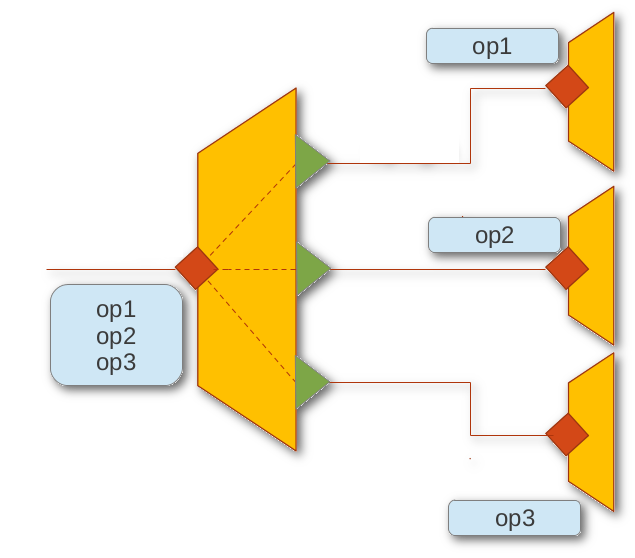
\includegraphics[width=0.6\textwidth]{pictures/aggregation.png}
    \caption{Aggregation is a generalisation of proxies and load balancers}
    \label{fig:aggregation}
\end{figure}


\section{The Jolie Engine and Interpreter}

In this section, the internals of the Jolie engine will be introduced. This
should give the reader the necessary knowledge to understand the changes made
to support a module and package system for Jolie.

At the core of the Jolie engine is the interpreter. Each interpreter is
responsible for parsing and executing a Jolie program. A single engine may run
several instances of the interpreter, this is most commonly the case when
embedding several other Jolie services.

A simplified view of the Jolie interpreter's pipeline can be seen in Figure
\ref{fig:jolie_pipeline}.

\begin{figure}[H]
\centering

\includegraphics[width=0.8\textwidth]{background/pipeline.eps}
\caption{A simplified view of the Jolie interpreter pipeline}
\label{fig:jolie_pipeline}
\end{figure}

The first phase of the interpreter is parsing the intent. In this phase the
interpreter will determine its purpose and, if any, modifiers to its ordinary
behavior.

The Jolie engine can be invoked from the command-line, the command-line is the
source of the intent which starts the first interpreter. The syntax for the
command line is (roughly) as follows: \txtl{jolie [commands and options]
    <program> [program arguments]}.

Options change the overall behavior of the engine, all interpreter instances
share these. These change the behavior of the interpreter.

Commands and program arguments, only belong to the interpreter that they were
originally passed. These determine what the interpreter will do.

The intent parsing phase is responsible for locating and retrieving the program
used.

A URI matching the input program is given to the program parser, the second
phase. The parser is responsible for creating the Abstract Syntax Tree (AST)
    which represents the input program. The parser will produce only a single
    root node, namely the \txtl{Program} node. Includes are thus implemented by
    essentially inserting the contents of the include target. A quirk for Jolie
    includes, is that relative file includes are not resolved relative to the
    current file, but rather to the current working directory (i.e. where the
            engine was started).

The third phase traverses the AST to make sure that it is semantically valid.
This weeds out programs that are syntactically correct, but not semantically
valid. The checks performed in this phase are somewhat limited, given the
dynamic nature of the language.

Given a semantically valid AST the interpreter is ready to build the
interpretation tree. The interpretation tree contains new nodes, which are
runnable.

Once the interpretation tree is built, we're ready to execute the actual code
(which lives in the interpretation tree). The \txtl{CommCore} component is
responsible for all communication, we'll discuss this briefly when relevant.
Following its initialization, the user code of Jolie will start executing. The
\joliel{init} procedure is executed first followed by the \joliel{main}
procedure.

\section{A Complete Application with Jolie}
\label{sec:complete}

In this section we will describe a complete application written in Jolie. The
application will contain several services, and will be written using best
practices from before the module and package system.

Along the way several patterns used for re-using code will be highlighted. This
will serve as the core motivation for our solution.

\subsection{Architecture}

% Things we wish to cover in this section:
%
%   - Includes and why they will be problematic
%   - Configuring location of ports, both external and embedding of stuff
%   - Project structure, and why this is a problem
%   - Parameter configuration

The application we will be building is a very simple calculator system. The
architecture of our application is shown in Figure \ref{fig:complete_arch} we
see an illustration of the system's architecture.

The calculator service will provide various operations for applying an operator
on a sequence of numbers. In order to perform this, highly complex, action of
applying these operators, the calculator will contact other microservices.

The dashed region (TODO) displays services that should be running in the same
Jolie engine. This is accomplished via embedding, which was introduced in a
previous section.

\begin{listing}[H]
\begin{minted}{text}
+---------------+     +---------------+     +---------------------+
| web-calc      | --> | calculator    | --> | multiplication      |
+---------------+     +---------------+     +---------------------+
                              |
                              |
                              v
                      +---------------+
                      | addition      |
                      +---------------+
\end{minted}
\caption{The Architecture of a Simple Microservice System}
\label{fig:complete_arch}
\end{listing}

\subsection{Implementing the Calculator Service}

We will keep our focus on the \emph{calculator} service, and its interacting
with other services. Putting together the stuff learned from the previous
sections, we can quickly setup an input port for the service, which has the
appropriate interface. It is considered best practice to place the public
interfaces that a service exposes in its own separate file. Files intended for
other services to include typically have the file extension \verb!.iol! as
opposed to \verb!.ol!. There is no technical difference between the two, but it
allows for the developer to more easily express intent. Files that are included
can be placed in the \verb!include! directory, this directory is always
implicitly added to the search path.

Thus in order to implement our calculator service we create two files, one for
the service implementation (\verb!calculator.ol!), and another which can be
used by other services (\verb!calculator.iol!). The implementation and
interfaces are shown in Listing \ref{lst:simple_start}.

\begin{listing}[H]
\begin{multicols}{2}

\begin{minted}[breaklines,fontsize=\footnotesize]{jolie}
// calculator.ol
include "console.iol"

inputPort Calculator {
    Location: "socket://localhost:12345"
    Protocol: sodep
    Interfaces: ICalculator
}

main {
    [sum(request)(response) {
        println@Console("Implementation goes here")()
    }]

    [product(request)(response) {
        println@Console("Implementation goes here")()
    }]
}
\end{minted}

\columnbreak

\begin{minted}[breaklines,fontsize=\footnotesize]{jolie}
// calculator.iol
type Numbers: void {
    .numbers[2, *]: int
}

interface ICalculator {
    RequestResponse:
        sum(Numbers)(int),
        product(Numbers)(int)
}
\end{minted}
\end{multicols}
\caption{TODO Caption}
\label{lst:simple_start}
\end{listing}

\begin{observation}
    The interfaces and types of a service are typically separated into their
    own files. This files typically has the extension \verb!.iol! to indicate
    that it does not contain a service implementation, but is rather intended
    for inclusion by a service which requires it.

    This file is typically put in the \verb!include! directory. This directory
    is always added to the search path natively by the Jolie engine.
\end{observation}

The operations that the calculator exposes, needs to collaborate with the other
services. In order for us to speak to them they need output ports.

First of all the output ports needs interfaces. Like we did with the calculator
service, the other services have exposed their interfaces in a special file
intended for inclusion. As a result we will have to copy the
\mintinline{text}{.iol} files of these services into our own.

Secondly these output port needs to be reached. We can either embed the
services, making it run inside of the same Jolie engine as our calculator
service, or we can provide external bindings to it. For output ports we may
change this binding dynamically at runtime. Note that this is unlike input
ports which must be ready at deployment time.

Binding an output port to an external service is relatively easy. For example
to let the \verb!multiplication! port bind to a service using https, we might
write \mintinline{jolie}{Location: "socket://mult.example.com:443"} and
\mintinline{jolie}{Protocol: https}. The input port at the multiplication processor
would also have to match this, to ensure it runs on the correct port and speaks
the correct protocol.

It is a similar to bind an output port to an embedded service. However this is
done by setting the \mintinline{jolie}{Location} or \mintinline{jolie}{Protocol}
attributes. We must instead instruct the engine to embed the service, which
most importantly requires us to point to some executable service. The Jolie
engine supports several language for these embedded services, including Jolie,
Java, and JavaScript. For our desired deployment, we wanted to embed the
addition service inside of the calculator service. Assuming that the addition
service is written as a Jolie service, and its service is implemented in
\mintinline{text}{addition.ol}, then we may create an embedding as shown in
Listing \ref{lst:simple_embedding}. Just like in the case of the external
services, the input port of the receiving service \emph{must match}. In the
case of embedded service there must be an input port listening on the
\mintinline{jolie}{"local"} location.

Quite often the location of an input port is considered a deployment problem.
We see this quite clearly in the case of embedding a service. All current
solutions in Jolie, require us to \emph{modify the source code of a service},
simply to change where the service should listen. Best practices in Jolie
attempt to make this less of a problem by including a configuration file which
contains constants. The addition service, might include a file called
\verb!addition.iol! with constants setting up the location and protocol
of the service. An example of this is shown in Listing
\ref{lst:include_as_conf}.

\begin{listing}[H]
\begin{multicols}{2}

\begin{minted}[breaklines,fontsize=\footnotesize]{jolie}
// addition.ol
include "addition.iol"

inputPort Addition {
    Location: ADDIITON_LOCATION
    Protocol: ADDIITON_PROTOCOL
}
\end{minted}

\columnbreak

\begin{minted}[breaklines,fontsize=\footnotesize]{jolie}
// addition.iol
constants {
    ADDIITON_LOCATION = "local"
    ADDIITON_PROTOCOL = sodep
}
\end{minted}

\end{multicols}

\caption{A common Jolie practice for solving configuration of a service, is to
    include a file containing constants with the desired configuration.}

\label{lst:include_as_conf}

\end{listing}

\begin{observation}
    Most configuration of Jolie services are done via constants. Jolie
    constants, different from most other languages, can be simple literal
    types, or they may even contain identifiers. This makes them rather
    versatile in what they may configure.

    The constants are placed in a separate source file, which is included by
    the service requiring the configuration.
\end{observation}

\begin{listing}[H]
\begin{minted}{jolie}
embedded {
    Jolie:
        "addition.ol" in Addition
}
\end{minted}

\caption{Embedding the \mintinline{jolie}{addition} service in the
    \mintinline{jolie}{Addition} output port}

\label{lst:simple_embedding}

\end{listing}

With the code from Listing \ref{lst:simple_start} where the output port
\mintinline{jolie}{Console} is defined. The output port points to an embedding
of the console service, and is included directly in the \verb!console.iol!
file. This is a fairly common pattern used in Jolie, especially for services
that work in a library-like fashion (i.e. not intended as a stand-alone
service). This pattern is used for almost every single service in the Jolie
standard library.

\begin{observation}
    Services intended to be used as libraries are often contained in a single
    \verb!.iol! file. This file contain everything required to set it up,
    included interfaces, types and an embedded output port.

    This makes it very easy to use the service, however it also makes it
    impossible to bind to this service externally, without first getting an
    embedding. This isn't possible since we cannot include the interfaces and
    types by themselves.
\end{observation}

With the output ports correctly configured, we may now implement the actual
business logic for our calculator. For completeness sake this might look like
shown in Listing \ref{lst:op_impl}.

\begin{listing}[H]
\begin{minted}{jolie}
[sum(request)(response) {
    total = 0;
    for (i = 0, i < #request.numbers, i++) {
        // Add current number with total, and store result in total
        add@Addition({
            .a = total,
            .b =  request.numbers[i]
        })(total)
    };
    response = total
}]
\end{minted}
\caption{Implementing the checkout operation}
\label{lst:op_impl}
\end{listing}

Finally we want to reflect slightly on the file structure that this service
ended up having. In order to use external services, we had to include files
which contain these interfaces. This version is worse when an embedding is
desired, since the entire service with its implementation is suddenly required.

The files from these external service are also hard to manage. It isn't
possible to simply move the source code of a service into its own directory.
This is not possible since includes, unlike in most other languages, are not
relative to the file performing the include, but rather relative to the project
level root. Thus if we wish to move the service to a new directory, all
includes in the source code would have to be updated. A common result of this
is that every single file gets dumped into the project level root. When all
files are stored in the same directory, we also get a much larger chance of
having name conflicts. As a result names tend to become rather large, to make
it less likely that a conflict occurs.

The final file structure of the calculator service is shown in Listing
\ref{lst:file_structure}.

\begin{listing}[H]
\begin{minted}{text}
.
+-- include
|   +-- calculator.iol
|-- addition.iol
|-- addition.ol
|-- multiplication.iol
+-- calculator.ol
\end{minted}
\caption{File structure of the calculator service}
\label{lst:file_structure}
\end{listing}

\begin{observation}

    In order to collaborate with other services, it is often needed to manually
    copy files into the service. The files required depend on if an embedding
    is required, when an embedding is required we will need the entire service
    (and any services it may depend on itself). If we just need to interface
    with it, we can simply include the files required for its interface files.

    Structuring the files is problematic, due to \verb!include! statements not
    being relative to file performing inclusion.

\end{observation}




\chapter{Jolie Modules}
\section{Modules: Design and Implementation}

A module in Jolie is defined as a project root directory, and optionally an
entry-point. Modules are uniquely identified by a name.

The Jolie engine needs to know about these modules. The engine is informed
about these modules from the intent, passed as options, which starts the
engine. This information is collected in the ``intent parsing'' phase, and is
made available to any later phase that might need it.  Since the intent is
passed as an option, all interpreter instances inside the engine will know
about each module.  As a result any embedded service will also be aware of the
same modules.

As an example, we may inform the engine about a module called ``foo'', which
has its source code placed in \verb!/packages/foo!  with an entry-point in
\verb!/packages/foo/main.ol! we would write: \mintinline{text}{--mod
foo,/packages/foo,main.ol}. This implementation technique is very close to
how, for example, you would add a JAR file to the classpath of a Java program.
% TODO Very informal argument

The result of this decision is that quite a lot of additional options may need
to be passed to the engine. However this choice was purposely chosen, it is
left for another tool to make this job easier. In this case a package manager
is expected to take the heavy lifting, and figure out which modules exists.
This allows for more freedom in how these tools are implemented, and another
implementation strategy, than the one provided in the package manager, could be
created without any changes to the language infrastructure. See Section TODO
about how the package manager passes this information to the engine.

To allow for better organization, a new type of include has been added to the
language. These include allows the developer to include from a particular
package. The syntax of this include is shown in Listing \ref{lst:mod_include}.
When a package include is used, the search path will be altered, such that the
project root is changed to that of the package (as opposed to where the engine
was started). Any file included from within this package should perform its
includes relative to its own root, rather than the project root.

TODO Example

The new include syntax, along with native support for modules, allows for the
code to properly organized. With this a module may be placed inside of its own
directory, without any of the code having to be changed.

\begin{listing}[H]
\begin{minted}{jolie}
include "<file>" from "<module>"
\end{minted}
\caption{Extension to the include statement, made for module imports}
\label{lst:mod_include}
\end{listing}

\subsection{Include Algorithm for Jolie}

TODO To this date I still don't understand how the include algorithm works. Ask
Fabrizio about this.

\subsection{Module Include Algorithm}

TODO Module includes modify the search path. This also means the injection of
the include directory, which is used as a convention. This helps maintain
expected behaviour.

TODO In order to implement the root switching we use a stack.

\section{Configuration}
\label{sec:col}

From Observation 2 we saw that most configuration was done via the inclusion of
source code. This source code would expose constants (read: literal values
\emph{and} identifiers). The included source code, however, can do anything
that Jolie source normally can, and is not limited to just the desired
configuration. As a result, a service developer cannot be certain that the
configurator (entity providing configuration) doesn't start messing with
other details of the program. Deploying defensive
programming\footnote{Defensive programming techniques are usually employed for
systems that require high availability, or where safety and security is
required\autocite{Jon05}.} techniques against this becomes significantly more
problematic, since no guarantees about the configuration source file can
be made.

Distributing re-useable packages is problematic with this approach. Common
features of package managers expect the source code of packages to be
read-only, for example, when updating packages. Without this property,
    source-code merges would be required.

This gives us plenty of reason to explore the need for a native configuration
format.  Most other systems would most likely go for a system defined in user
code, as opposed to natively. An example of such framework, is Vert.x, a
tool-kit for building reactive applications on the JVM.  Examples of such
``reactive applications'' are microservices. The configuration workflow of
Vert.x\autocite{VERTA} is shown in Figure \ref{fig:normal_conf}. The system
will retrieve, and read external configuration files, directed by the user
code, and apply the configuration as needed.

% Most other systems can do this at run time
% For example Vert.x does this by reading external configuration files
% Once configuration is done, we can start up the server

\begin{figure}[H]
\centering

\includegraphics[width=1.0\textwidth]{modules/normal_conf.eps}
\caption{Simplified workflow for configuration of Vert.x applications}
\label{fig:normal_conf}
\end{figure}

% http://vertx.io/blog/vert-x-application-configuration/
% http://vertx.io/docs/vertx-config/kotlin/

However, it is not straight forward to implement such a system in Jolie.
In general-purpose languages, the constructs (such as a server's socket) for
the microservice architecture are created in user code. As a result they are
entirely accessible from user code. This make it feasible to change their
behaviour, since code can run before deployment occurs.

In Jolie, the constructs are managed directly by Jolie. This has multiple
advantages, such as less complexity in user code, but Jolie user code also
loses power in the process. For example, a Jolie program cannot control the
network directly, but must instead use the abstractions provided by the
language (message-passing).

The primary need for a native solution comes from input ports. Input ports in
Jolie require their values to be set at deployment time. It is not possible to
reconfigure their location during runtime, and for good reasons. TODO Reasons
can't come up with any right now.

Additionally, creating a native solution provides many opportunities in terms of
creating more powerful features. For example, the configuration format allows
us to easily move between embedding a service, and binding to an external
service.

\subsection{Introducing the Jolie Configuration Format}
\label{sec:conf_units}

In the coming section we will cover the Jolie Configuration Format (file
extension: \txtl{.col}).

% Goals

This new configuration format should allow a developer to provide configuration
for a service, which works in the setting of packaged services. This will
entirely replace the old system of using a mix of constants and hard-coded
values.

The configuration system will only allow configuration of constructs which has
been marked as such by the module. This should also allow a developer, and
potentially tools, to quickly identify which constructs allow configuration.
As much as possible, the code should act as documentation of itself.

Additionally the system should work with the existing checking tools (e.g. the
\txtl{--check} flag). The checking tools of Jolie are, for example,
used by editor plugins to show errors. These checks do not execute
any code. The checking algorithm should check that the provided
configuration is valid.

% Basic concepts and example

A configuration file is build up of \emph{configuration units}.  A
configuration unit is the basic entity, which encapsulates the configuration of
a single Jolie module.

A unit is uniquely identified by its profile name and module. Having multiple
profiles for the same module can be useful for a variety of use-cases. A common
use-case, for example, could be separate profiles for development and
production.

The units can hold configuration for every possible type of configurable
construct in Jolie. The configuration format support the following constructs:

\begin{enumerate}
    \item Input and output ports
        \begin{itemize}
            \item Location
            \item Protocol and protocol parameters
            \item Embedding of other services (output ports only)
        \end{itemize}
    \item General purpose parameters (values accessible from
            Jolie programs)
    \item Interface rebinding
\end{enumerate}

We'll start by introducing the configuration format through examples.  The
configuration format is custom, and made to mimic the syntax of Jolie. This
decision was chosen to make it easier to convert existing Jolie code.

Listing \ref{lst:simple_conf} shows a simple configuration unit. This
units sets the location and protocol for the output port \joliel{A} (line 3 and
        4), the location of the input port \joliel{ModuleInput} (line 8), and
two parameter assignments (line 11 and 12).

\begin{listing}[H]
\begin{minted}{jolie}
profile "hello-world" configures "my-module" {
    outputPort A {
        Location: "socket://a.example.com:3000"
        Protocol: sodep { .keepAlive = true }
    },

    inputPort ModuleInput {
        Location: "socket://localhost:80"
    },

    myParameter = 42,
    myParameter.subProperty = "hello"
}
\end{minted}

\caption{A simple configuration unit named \joliel{hello-world}
    configuring the module \joliel{my-module}}

\label{lst:simple_conf}

\end{listing}

Embedding of output ports can be performed from within a configuration unit.
This moves the embedding from being a code problem to, what it should have
been, a deployment problem.

Listing \ref{lst:conf_embedding} shows the embedding of output port \joliel{A}.
Note that we need to make a reference to the module (line 2), since the profile
names are placed under a namespace for each module. This way multiple services
can share the same name, a situation which is likely to occur with common
profile names, such as ``development'' and ``production''.

\begin{listing}[H]
\begin{minted}{jolie}
profile "hello-world" configures "my-module" {
    outputPort A embeds "a-module" with "a-profile"
}

profile "a-profile" configures "a-module" {
    // configuration of a-module goes here.
}
\end{minted}
\caption{Embeddings make reference to other configuration units}
\label{lst:conf_embedding}
\end{listing}

As seen in the examples, providing partial configuration, as opposed to
complete configuration, is allowed. In certain cases, partial configuration is
provided because the remaining values are defined by the module itself. In
other cases, partial configuration is provided due to the extension of other
profiles.

A configuration unit may extend another unit. The two, however, must configure
the same module. The inheritance tree may be of an arbitrary depth, but
each unit may only extend a single unit, and they must configure the same
module.

If the child and parent disagree on configuration, the child always decides.
For example, if unit ``B'' extends ``A'', and they both configure the same
value, then the constructs found in B are the ones that are used. Listing
\ref{lst:conf_extends} shows an example of inheritance.

\begin{listing}[H]
\begin{minted}{jolie}
profile "a" configures "a-module" {
    aValue = 42,
    aValue.sub = "hello",

    outputPort ExternalService {
        Location: "socket://external.example.com:42000"
    }
}

profile "b" configures "a-module" extends "a" {
    aValue = 100
    // aValue.sub = "hello"
    // ExternalService.location = "socket://external.example.com:42000"
}
\end{minted}
\caption{Configuration units may extend other units}
\label{lst:conf_extends}
\end{listing}

The module developer is often aware of what the default configuration should
be.  For this, default configuration profiles can be shipped along the modules.
The default configuration units are implicitly imported into every
configuration file which uses a particular module.  The Jolie engine will look
for any \txtl{.col} file in the \txtl{conf} folder. This folder should be
placed relative to the module's root. For example, if module "a" has a file
called \txtl{conf/my-defaults.col}, which contains a unit called "default".
Then the user of the package may either write a configuration unit which
extends this, simply by writing \joliel{profile "something" configures "a"
    extends "default"}, or the default directly. There is no need for any
    inclusion of this file.

While no configuration unit is required to be complete, the one used by the
engine must be complete. If an interpreter is instructed to use a partial
configuration unit an error will be produced.

\subsection{Input and Output Ports}

Input and output ports, both existing constructs, are defined just like before
in the Jolie code.

Externally configurable ports are created by leaving out fields that should be
configurable. Listing \ref{lst:configurable_input} shows a configurable input
port.

Only the fields which are not already listed become configurable. This is
useful when building a service that needs to make assumptions about its input
ports. For example, if a developer is building a generic web-server, it is
useful to allow the developer to change the location, but the protocol should
remain fixed.

One typical assumption that Jolie services make about their input ports come
from aliases that are made in the protocol configuration, an example is shown
in line 4 of Listing \ref{lst:configurable_input}. The pointer statement takes
two variable paths and makes the one on the left link to the one on the right.
The result of this is setting \txtl{statusCode} will cause the HTTP status code
It should also be noted that the configuration units \emph{do not} support
aliases, and there are no other ways of accessing variables hidden in the
protocol configuration. As a result, any service which needs to do something
special with its protocol configuration, like aliasing, must do it in source
code. Since the aliased variable now also takes on a new semantic meaning, it
also makes sense that it must be named directly in source code, and not left to
configuration, where it could take any arbitrary name.

\begin{listing}[H]
\begin{minted}{jolie}
inputPort MyWebServer {
    Protocol: http {
        .keepAlive = true;
        .statusCode -> statusCode;
    }
    Interfaces: MyWebServerInterface
}
\end{minted}
\caption{A bare-bones configurable input port for a web-server}
\label{lst:configurable_input}
\end{listing}

However, simply leaving out fields, and assuming they must be configurable
proves somewhat problematic for output ports. Output ports require no fields,
other than the interfaces, to be defined at deployment time. It is quite
common for dynamic ports to not add a default location or protocol,
assuming it is changed before use. To deal with this problem, it was
decided to add a new keyword (\joliel{dynamic}) for output ports which
need to change their location and protocol dynamically. Only output
ports marked with this keyword are allowed to be changed at run-time.
Dynamic ports are also not configurable.

\subsection{Parameters}

Parameters are read-only values which are provided to a Jolie module at
deployment time. A parameter is type-checked at deployment time, to ensure that
its type matches what the underlying service expects. Listing \ref{lst:params}
shows a parameter definition and its use.

The type-checking feature functions both as a mean of documentation and
ensuring that the supplied configuration is valid. Like any other type-checked
feature of Jolie, it is possible to opt-out simply be setting the type to be
\txtl{undefined}.

\begin{listing}[H]
\begin{multicols}{2}
\begin{minted}[breaklines,fontsize=\footnotesize]{jolie}
// service.ol
parameters {
    myParameter: string {
       .foo: int
       .bar: bool
    }
}

main {
    println@Console(myParameter)(); // "Root"
    println@Console(myParameter.foo)(); // 42
    println@Console(myParameter.bar)() // false
}
\end{minted}

\columnbreak

\begin{minted}[breaklines,fontsize=\footnotesize]{jolie}
// service.col
profile "my-profile" configures "service" {
    myParameter = "Root",
    myParameter.foo = 42,
    myParameter.bar = false
}
\end{minted}

\end{multicols}
\caption{A parameter definition and its use}
\label{lst:params}
\end{listing}

From a high-level point of view, parameters are very similar to constants.
However parameters weren't implemented as an extension of constants due to the
implementation of constants. Namely, constants aren't implemented using the
``Value'' system, which is used by all variables and messages in Jolie, but
rather implemented at the parser level.

When the Jolie parser encounters a constant definition, it will save the token
from the assignment and associate it with the identifier on the left-hand side.
Only identifier tokens and simple value tokens are allowed. The constant
definitions are limited to only a single token. As a result, it is not possible
to define more advanced tree-like values, which parameters such as
\joliel{myParameter} from Listing \ref{lst:params} would require.

Whenever the parser reaches a place where a constant would be allowed, it will
look at the next token, check if it is an identifier, and try to replace the
current token with the token defined by the constant. This produces some rather
surprising results and has limitations, which is not commonly found in other
programming languages.  Listing \ref{lst:jolie_constants} illustrates how the
Jolie parser processes constants.

\begin{listing}[H]
\begin{multicols}{2}

\begin{minted}[breaklines,fontsize=\footnotesize]{jolie}
constants {
    FOO = 42
    BAR = ActualInterface
}

init {
    println@Console(FOO)()
}

courier Foo {
    [interface BAR(req)(res) {
        /* ... */
    }]
}
\end{minted}

\columnbreak

\begin{minted}[breaklines,fontsize=\footnotesize]{jolie}
init {
    println@Console(42)()
}

courier Foo {
    [interface ActualInterface(req)(res) {
        /* ... */
    }]
}
\end{minted}

\end{multicols}

\caption{Constants in Jolie works by replacing tokens at the parser level.
    Left: The input program. Right: The program which the parser ends up
        seeing}

\label{lst:jolie_constants}

\end{listing}

While it would have been possible to extend the value system to support values
it was ultimately decided against. Adding both optional type-checking of
constants and expanding to values was seen as too big a departure from the
original intent of constants. For backward compatibility reasons constants
would also still not have been pure values, but rather either an identifier or
a value.

The new parameters block is an addition to the AST of Jolie programs. This
addition currently only works in collaboration with the configuration and
module system. The block is simply not valid to use without. If any parameter
is not defined by configuration or has the wrong type the checking scripts of
Jolie will throw an error.

Even though the parameters block is added to the AST it will not be visible in
the final interpretation tree. We'll learn more about this in Section
\ref{sec:col_impl}.

\subsection{Interface Rebinding}
\label{sec:interface_rebinding}

TODO Need to be more explicit about which features are new, and which are
existing features.

In this section we will first more closely inspect the existing aggregation,
   and courier features of Jolie. This leads to the introduction of interface
   rebinding which is explained following that.

Jolie provides the ``aggregation'' feature. We first introduced aggregation in
the background material for Jolie. In short the feature is a generalisation of
proxies. The aggregation feature simply forwards requests from one service to
another. A simple proxy to the calculator service is shown in Listing
\ref{lst:aggregation_example}.

\begin{listing}[H]
\begin{minted}{jolie}
include "calculator.iol" from "calculator"

inputPort Self {
    Location: "socket://localhost:12345"
    Protocol: sodep
    Aggregates: Calculator
}

outputPort Calculator {
    Location: "socket://calc.example.com:12345"
    Protocol: jsonrpc
    Interfaces: ICalculator
}
\end{minted}

\caption{A calculator proxy: This service will proxy any call to the calculator
    service bound in the output port \joliel{Calculator}}

\label{lst:aggregation_example}

\end{listing}

Aggregation can be extended by using couriers, which allows for the service to
run code associated with requests that are proxied. Couriers may work either
for an entire interface, or any particular operation. A courier may even
decide not to forward a particular call. Listing \ref{lst:simple_courier} shows
an extension for the calculator proxy with a courier.

\begin{listing}[H]
\begin{minted}{jolie}
courier Self { // The name of a courier matches its input port

    // Couriers can match an entire interface
    [interface ICalculator(request)(response) {
        println@Console("Received call for calculator!")();
        forward(request)(response)
    }]

    // Or just a particular operation
    [sum(request)(response)] {
        // The courier may choose to forward a request, or answer the
        // request itself
        if (#request.numbers > 2) { forward(request)(response) }
        else { response = request.numbers[0] + request.numbers[1] }
    }
}
\end{minted}

\caption{A courier allows additional code to run alongside a potential
    forwarding}

\label{lst:simple_courier}

\end{listing}

Additionally Jolie supports ``interface extenders''. These can, like the name
suggests, extend the types of operations (in interfaces) with additional
fields. These may add additional fields for every operation, or specific
operations. These can also add faults to the type signature of an operation.

Like with any other output port, the service relies entirely on the interface
listed in the output port to be correct. There is no communication with the
target service about the correct interface. If the interface doesn't match, it
will simply fail when attempting to invoke the operation.

\emph{A consequence of this is that it isn't possible to create entirely generic
proxies without knowing the interface.}

The aggregates and courier features allow for Jolie to implement many different
common proxy-like patterns. These patterns mostly deal with their target
service in a generic fashion, making very few, if any, assumptions about the
target service. However because the aggregations feature needs the interface it
would be impossible to write a fully generic proxy service.

The interface rebinding feature fixes this problem, by allowing configuration
files to redefine an interface at deployment time. This way the generic service
may write ordinary code, making no assumptions about the underlying service,
and only at deployment time it will know which interface the target service
has.

\begin{listing}[H]
\begin{minted}{jolie}
interface ITarget
\end{minted}
\caption{Configurable interfaces are defined by leaving the body empty}
\label{lst:ext_interfaces}
\end{listing}

The interface is bound from the configuration file, in a similar fashion to
other configurable units, as shown in Listing \ref{lst:reconf_interface}.

\begin{listing}[H]
\begin{minted}{jolie}
interface ITarget = ICalculator from "calculator"
\end{minted}

\caption{Rebinding the \joliel{ITarget} interface to the \joliel{ICalculator}
    interface from the calculator module}

\label{lst:reconf_interface}
\end{listing}



\subsection{Syntax of the Configuration Format (COL)}

In this section the formal grammar of the configuration format is presented.
The grammar is presented in a ABNF-like syntax. Complete syntax is presented in
Appendix 2.

All literals are case sensitive.

A configuration file starts by a list of includes, followed by a list of
regions, as shown in start rule \mintinline{abnf}{configuration-tree}.

\begin{minted}{abnf}
configuration-tree = *include *region

include = "include" qstring

region = region-header "{" region-body "}"
region-header = [ "profile" qstring ] "configures" qstring
                [ "extends" qstring ]
region-body = *definition
definition = port | interface | parameter
\end{minted}

The definitions inside of a region correspond to the different configurable
units. The syntax is made to closely mimic the syntax of existing Jolie code.

\begin{minted}{abnf}
port = input-port | output-port
input-port = "inputPort" identifier "{" port-body "}"
output-port = embedded-output-port | external-output-port
external-output-port = "outputPort" identifier "{" port-body "}"
embedded-output-port = "outputPort" identifier "embeds" qstring
                       "with" qstring
port-body = *port-property
port-property = location-property | protocol-property
location-property = "Location" ":" qstring
protocol-property = "Protocol" ":" identifier [ protocol-config ]
protocol-config = inline-tree

interface = "interface" identifier "=" identifier "from" qstring

parameter = variable-path "=" value
variable-path = var-id *var-node
var-id = ( "(" qstring ")" ) | identifier
var-node = "." var-id [ "[" unsigned-int "]"  ]
value = ( primitive [ inline-tree ] ) | inline-tree
inline-tree = "{" *(tree-child ",") tree-child "}"
tree-child = "." variable-path "=" value
primitive = qstring | int | long | double | bool
\end{minted}

The values very closely resemble what Jolie allows, primarily just removing
variables from the syntax. Variable identifiers can be strings, like in Jolie,
to allow for special variable names which would otherwise not be
valid identifiers. This is primarily useful for building dictionary like
structures with arbitrary string keys.

Additional configuration file supports C-style comments, these are allowed
anywhere and are simply ignored.

\begin{minted}{abnf}
comment = single-line-comment | multi-line-comment
single-line-comment = "//" <any text except line breaks>
multi-line-comment = "/*" <any text except "*/"> "*/"
\end{minted}


\section{Implementing the Configuration Format}
\label{sec:col_impl}

The new interpreter pipeline is as follows, new phases marked in bold text:

\begin{enumerate}
\item Intent parsing
\item Jolie code parsing
\item \textbf{Configurator}
\item Semantic verifier
\item Interpretation tree builder
\item \textbf{Late verification}
\item Communication core init
\item Init \& main process
\end{enumerate}

The primary work occurs in the configurator service, but some of the
verification work, namely the parameters, are postponed until after the
interpretation tree has been build.

\subsection{The Configuration Phase}

The configuration phase builds upon the result of the intent and parsing phase.
From the intent phase we receive information about modules and the intent to
use a certain configuration unit. From the parsing phase we obviously get the
AST.

The configuration phase works by modifying the AST to insert the configuration
gathered from the configuration unit. The processed AST is handed to the later
phases, and the remainder of the pipeline works mostly like it has before.

\subsubsection*{Processing of Configuration Files}

\paragraph{Resolving configuration files}

The first step of the configurator is to gather a fully processed configuration
unit. This process starts by looking for the configuration file which was
passed from the intent. The configuration unit is passed with:
\\\txtl{--conf <unitName> <filePath>}.

If the file path is an absolute file path, then that file will always be used.
However if the file path is relative some searching is required. The base case
for resolving this is to look for the configuration file relative to the
current working directory. However this approach stops working once modules starts
embedding other modules in a static fashion.

Consider three modules, each providing one service, \txtl{A} and \txtl{B},
\txtl{C}. Module \txtl{A} depends on \txtl{B}, and \txtl{B} depends on
\txtl{C}.

\begin{listing}[H]
\begin{minted}{jolie}
/* /a/main.ol */
outputPort B { Interfaces: BInterface }

/* /a/config.col */
profile "a-deployment" configures "a" {
    outputPort B embeds "b" with "b-deployment"
}

profile "b-deployment" configures "b" { /* ... */ }

/* /b/main.ol */
outputPort C { Interfaces: CInterface }

embedded {
    Jolie:
        "--conf c-deployment embedded.col c.mod"
}

/* /b/embedded.col */
profile "c-deployment" configures "c" { /* ... */ }
\end{minted}

\caption{Relevant source code for modules \txtl{A} and \txtl{B}. Each file
    marked by a comment, placed in a directory corresponding to their module.
        For example \txtl{/a/main.ol} is the \txtl{main.ol} file which belongs
        to the module \txtl{A}}

\label{lst:need_for_parent}

\end{listing}

Relevant code is shown in Listing \ref{lst:need_for_parent}.  Assume that we
start module \txtl{A} with \\\txtl{--conf a-deployment config.col a.mod}.  The
problem arises because the fixed embedding of module \txtl{C} performed in
\txtl{B}. Because the files are resolved relative to working directory in which
the engine was started, the engine would look for the configuration file in
module \txtl{A}. To fix this, every time an embedding is performed the engine
will implicitly add a \txtl{--parent} flag. This flag informs the new
interpreter who performed the embedding. If the parent flag has
been given, the configuration file will be found relative to that of the
parent.

Working directory, throughout this is \txtl{/a/}.  The following will happen:

\begin{enumerate}

\item Start engine (from CLI) with: \txtl{--conf a-deployment config.col a.mod}
File resolved to \txtl{/a/config.col} because of relative path and no parent.

\item Configuration causes embedding of \txtl{b-deployment} with:
\\\txtl{--parent a --conf b-deployment /a/config.col b.mod}. File resolved to
\\\txtl{/a/config.col} because of absolute path.

\item Source embedding in \txtl{B} causes embedding of \txtl{c-deployment}
with: \\\txtl{--parent b --conf c-deployment embedded.col c.mod}. File resolved
to \\\txtl{/b/embedded.col} because of relative path with parent.

\end{enumerate}

\paragraph{Parsing of configuration files}

With the configuration file resolved, it is passed to the configuration parser
along with a list of known modules. The parser follows the conventions
established by the existing Jolie code parser. The parser is a hand-written
recursive descent parser with one token lookahead.

The parser directly outputs the AST. At the top level the AST consists of
\javal{Region}s which directly map to the configuration unit abstraction. Each
\javal{Region} are namespaced under the module that they configure. Internally
each namespace maps the name of the \javal{Region} to the actual
\javal{Region}. The top-level node of the AST contains a dictionary mapping
between the name of modules and their namespaces. The Java type for this
mapping ends up being \javal{Map<String, Map<String, Region>>}, this allows for
easy access of \javal{Region}s when they are needed. This does however also
mean that duplicates must be caught during parsing, since they would otherwise
just silently override previous entries. This would typically have been
performed in a later stage to keep the parser ``pure''. In this case some
purity was sacrificed for some efficiency and ease of use.

The grammar of the configuration format closely follows the grammar of Jolie
code. As a result the configuration format also re-uses AST nodes where
possible. As we will see later, this proved helpful when outputting a
configured AST. The configuration grammar only supports a subset of the
features that Jolie code does.

Recall from Section \ref{sec:conf_units} that each module may publish default
configuration units, which can be used by user-level configuration units. For
this reason the parser will make special note of references to other
configuration units. Such references currently only appear in output port
embeddings (e.g. \\\joliel{outputPort Foo embeds "foo" with "a-foo-unit"}).

Once the initial file has been parsed, every single configuration file placed
in the ``conf'' directory of referenced modules are parsed and placed in the
same AST. Configuration files parsed during this phase may itself have
references to other modules, in that case these will be pulled in as well.  A
set of parsed defaults is kept to avoid parsing the same file multiple times,
or potentially infinite loops.

\paragraph{Merging configuration files}

With the entire configuration tree in place, merging is performed to create a
single \javal{Region} which represents the actual configuration. The merging
occurs between a \txtl{child} and its \txtl{parent} region (that is, the one it
        extends, if any) and results in a \txtl{merged} region. The
\txtl{parent} is always merged (via a recursive call) first. The first
\txtl{child} selected is the \txtl{Region} matching the profile name and
package given by the intent.

For ports, the merging algorithm works by inserting all the ports of the
\txtl{child} into the \txtl{merged} region. The ports of the \txtl{parent} are
then merged with the preliminary output of the \txtl{merged} region. The
process of merging a \txtl{port} of the \txtl{parent} against the \txtl{merged}
region is shown, in pseudo code, in Listing \ref{lst:merge_ports}. In short the
merging will favor the \txtl{child}, and the \txtl{parent} will only provide
values if the \txtl{child} doesn't.

\begin{listing}[H]
\begin{minted}[linenos=true]{text}
procedure merge(port: Port, merged: ConfigTree): Region {
    if (!merged.contains(port)) return port
    child = merged.getExisting(port)

    if (child.isComplete) return existing
    // The child cannot be an embedding, since those cannot
    // be partial.

    for (property in Port.properties) {
        if (child[property] == null) {
            child[property] = merged[property]
        }
    }
    return existing
}
\end{minted}

\caption{Pseudo code for merging a \txtl{parent}'s \txtl{port} into a
    \txtl{merged} configuration tree}

\label{lst:merge_ports}

\end{listing}

For parameters the same idea applies. However each parameter definition node in
the AST potentially only provides a partial value. For example the node
\joliel{foo.bar = 42}, where the type of \joliel{foo} is \joliel{string { .bar:
    int }}, only provides a partial definition of \joliel{foo}. For this reason
    the parameter assignments are first added from the \txtl{parent} and then
    by the \txtl{child}. This allows the definitions of the \txtl{child} to
    override those of the \txtl{parent}.

\subsubsection*{Applying Configuration to the AST}

The \txtl{merged} region from the previous section is then used along
with the AST corresponding to the Jolie program. The last phase of
the configurator will process the entire AST and output a new AST, which is
fully configured. This process works by running a \txtl{process} function on
every single top-level node. The \txtl{process} function will inspect the node,
and depending on the node return a list of replacement nodes.

Throughout this process the configurator will also verify that no configuration
is performed on nodes which aren't configurable. This includes dynamic ports
and non-empty interface definitions.

\paragraph{Ports}

When a port node is encountered in the AST, the \txtl{merged} region is
searched for an output port matching its name. If none is found, the AST node
is returned as it is, no modifications are made to it. Otherwise the
configuration proceeds. For input ports and non-embedding output ports the
process is the same. The properties of the AST port and the port represented in
the configuration region are compared one-by-one. If any property is defined by
both, an error is returned pointing to the AST node and the place that the
configuration took place. At the end, if no errors are returned, a new port is
returned with their properties merged together.

For output ports which embed another module the process is slightly different.
The configurator will first verify the existence of the configuration unit by
looking it up in the configuration tree. If it is not found an error will be
returned. Otherwise the configurator will output a new embedding node. The
embedding node will contain a reference back to the same configuration file the
current \txtl{Region} comes from. When the embedding is performed, the
configurator of the embedded service will lookup the correct configuration unit
from the same file. This will cause an addition parsing of the same
file, but a caching layer at the configuration parser could take care of this.
The embedding process is demonstrated in Listing \ref{lst:embedding_output}.

\begin{listing}[H]
\begin{multicols}{2}

\begin{minted}[breaklines,fontsize=\footnotesize]{jolie}
embedded {
    Jolie:
        "--conf foo-profile <inputConfigFile> foo.mod" in Foo
}
\end{minted}

\columnbreak

\begin{minted}[breaklines,fontsize=\footnotesize]{jolie}
outputPort Foo embeds "foo" with "foo-profile"
\end{minted}

\end{multicols}

\caption{AST nodes generated, shown as code (left), by configuration (right)
    for an output port containing an embedding}

\label{lst:embedding_output}

\end{listing}

\paragraph{Interface Rebinding}

Just like ports, when an interface definition is found the \txtl{merged} region
is searched for a matching interface definition. Assuming no errors, the
configurator must now replace the dummy interface definition with the real
interface definition as the configuration specifies.

Quickly recapping interface rebinding in the configuration is shown in Listing
\ref{lst:interface_rebinding_recap}. Note that the only information the
configurator has for locating the replacement is the name of the interface and
its module.

\begin{listing}[H]
\begin{minted}{jolie}
interface Dummy = Concrete from "my-module"
\end{minted}

\caption{Rebinding the interface \txtl{Dummy} to match the interface
    \txtl{Concrete} from the module \txtl{my-module}}

\label{lst:interface_rebinding_recap}

\end{listing}

The interface will be found by parsing the module's entry point. Its AST, if it
exists, will then be searched for an interface matching the replacement. Simply
replacing the dummy with its replacement, however, isn't enough. Consider, for
example, the scenario shown in Listing \ref{lst:interface_rebinding_types}. In
this scenario, the processed AST will no longer be valid due to the missing
types (\txtl{FooRequest} and \txtl{FooResponse}).

\begin{listing}[H]
\begin{minted}{jolie}
type FooRequest: void {
    .child: string
}

type FooResponse: int

interface Concrete {
    RequestResponse:
        foo(FooRequest)(FooResponse)
}
\end{minted}

\caption{Simply copying the interface definition is not enough, the types must
    also be copied}

\label{lst:interface_rebinding_types}
\end{listing}

The relevant type definitions are found by iterating through every operation of
the replacement interface. If the types listed in the operations are type links
those are followed. This leads to a recursive algorithm, which looks through
every type looking for type links, which will cause more types to be copied
over. In order to avoid infinite loops a set of already visited types is kept.
If a type has been seen before then its children will not be visited.

In the end, the original interface definition will be replaced, and all
necessary type definitions will also be added to the program.

\paragraph{Parameters}

Parameters being a new concept in Jolie simply outputs new nodes for every
single parameter assignment. This along with the definitions gathered from
ordinary Jolie code parsing are processed in the interpretation tree building
phase.

\subsection{Additions to the Semantic Verifier}

As we have seen several syntax changes were also made to the core languages.
These modifications to the syntax also slightly changed which programs were
legal. As an example, interfaces are now allowed to be empty at a syntactical
level, to signal that they should be replaced by configuration. However having
an empty interface not being replaced should still cause an error.

This means that additional checking must not be performed to ensure that
programs are semantically valid. Such a phase already exists in the compiler,
the semantic verifier.

The semantic verifier works by performing an AST traversal and validate the
semantics of each node.

The verifier has been updated to not allow empty interfaces, this was
previously enforced at a syntax level. Since the configurator runs before this
phase and updates the AST, this will only cause errors for non-configured
trees.

Non-dynamic ports are ensured to be constant by using features already
implemented by the semantic verifier.

The semantic verifier is the last phase of the Jolie interpreter when run with
the \txtl{--check} flag. As we will discuss in the coming section, it is not
practical to perform type-checking of parameters at this point.

\subsection{Additions to the Interpretation Tree Builder and Late Verification}

% Introduction

Interpretation tree building was expanded to support parameters. All other
features required no changes to AST structure, and could simply reuse existing
features.

This section will discuss the technical of how the Interpretation Tree Builder
(ITB) works. It will cover issues that are quite technical, and very specific
to this particular implementation of the Jolie engine.

% What is the ITB and what does it do?

The Interpretation Tree Builder (ITB) is the last step before a Jolie program
is ready to be executed. The ITB works by traversing the AST. The ITB will
collect information from the AST in the form of definitions and inform the AST
about their presence. These definitions include ports, interfaces, types, and
code procedures.

% Processes

Within code procedures the ITB will produce processes from the AST nodes which
are runnable. It is from processes the meat of code execution is implemented.
For example it is from processes everything from addition to operation calls
are implemented.

% When are types ready?

In this phase the ITB will be gathering complete information about types. Type
building is for the most part a one-to-one translation from the
AST nodes into the internal representation. An important job of the
ITB with respect to type building is resolving of type references. This turns
references to a type name into an actual reference to a concrete internal type.
Because types aren't build until this phase is what makes type-checking during
semantic verification problematic. The semantic verifier would essentially have
to duplicate the work of the ITB in order to perform type-checking earlier.
This also means that type-checking cannot be performed until the ITB is
finished.

% State, and how the ITB changes initial state.

The ITB will need to initialize the system with certain values. For example,
the ITB will initialize the \joliel{location} and \joliel{protocol} variables
of output ports. These variables are local only to a single request. At this
point, however, the state of the Jolie program has not yet been initialized.

In Jolie, state is associated with the current thread of execution. Jolie uses
a separate thread of execution for handling every message. As a result every
single request gets its own fresh state. All state is copied from the
initialization execution thread. This thread performs work requested by the ITB
followed by the \joliel{init} procedure. Thus right after the ITB is done, and
the initialization execution thread is started, code execution starts. This
includes both user code and loading of any embedded services.

It should be noted that any process which works with state must be run on an
execution thread, since it depends on the state being present on the thread.

% Handling of parameter definitions and assignments inside the ITB

The ITB receives two new node types from the configurator and code parser:
parameter assignments, and parameter definitions.

For parameter definitions the ITB will resolve the types. Ensuring that all
links are properly resolved. This will output a ``processed'' parameter
definition which the ITB will inform the interpreter about.

In a similar fashion, the ITB will process parameter assignments and inform the
interpreter. Type-checking cannot be performed at this point, due to types not
being ready before the ITB finishes. Simply outputting processes for
configuration will make it impossible to perform type-checking before code
execution starts, due to their dependency on state.

The processed assignments contains an ordinarily processed LHS, which contains
the variable path. The RHS has been processed into an expression, which can be
evaluated into a native Jolie value on which type-checking can be performed.

% Introduction of new phase and working around lack of state

Because of these constraints a new ``late-checking phase'' has been created.
This phase runs right after the ITB, but before code execution starts. In this
phase it is not possible to directly touch the init state. It is however
possible to both create values, and evaluate expression. This phase creates a
synthetic state by creating a new value, which will act as the state.
Expression are evaluated against this root and later type-checked. The result
of evaluating the parameter assignments are then copied into the init state,
   assuming, of course, that type-checking was successful.


\section{Examples}
\label{sec:module_examples}

In this section we will introduce two examples, which will showcase different
aspects of the Jolie module, and configuration system. These examples will be
revisited again in Section TODO, where they will be shown in the context of
packages.

\subsection{Example A TODO Name}

In this example we will look at the calculator example shown in the
introductory chapters. The calculator system will be updated to work under the
new Jolie module system. We will also show how what was previous problems that
required code changes, can now be performed entirely in independent
configuration files.

Quickly recapping from previous chapters.  Figure \ref{fig:simple_calc} shows
the system architecture for the calculator system. The system contains three
services. The main-point of contact for a client is the \txtl{calculator}
service. This service will delegate the ``hard'' work to the other two
services, that is \txtl{addition} and \txtl{multiplication}.

\begin{listing}[H]
\begin{minted}{text}
+----------------+     +--------------+     +----------------+
| multiplication | <-- | calculator   | --> | addition       |
+----------------+     +--------------+     +----------------+
      |
      v
+--------------+
| numbers      |
+--------------+
\end{minted}
\caption{System architecture for the ``calculator system''}
\label{fig:simple_calc}
\end{listing}

The file structure of our services contained a lot of duplication. The file
structure is shown in Listing \ref{lst:start_file_structure}. As we can see
from this there is quite a bit of duplication of files, and we cannot simply
copy the directories of our dependencies, as this would place the files in the
wrong places. We also resort to code files for distributing default
configuration profiles. Switching between embedding a service and binding to it
externally will also require significant changes.

TODO This uses the updated example from e-mail. The introduction needs to be
updated to use the same example.

\begin{listing}[H]

\begin{multicols}{3}

\begin{minted}[breaklines,fontsize=\footnotesize,frame=none]{text}
// multiplication
.
|-- multiplication.ol
|-- include
|   |-- mult_config.iol
|   `-- multiplication.iol
`-- numbers.iol

// numbers
.
|-- include
|   `-- numbers.iol
`-- main.ol
\end{minted}

\columnbreak

\begin{minted}[breaklines,fontsize=\footnotesize,frame=none]{text}
// calculator
.
|-- addition_config.iol
|-- addition.iol
|-- addition.ol
|-- calculator.ol
|-- include
|   `-- calculator.iol
|-- mult_config.iol
|-- multiplication.iol
|-- multiplication.ol
|-- numbers.iol
`-- numbers.ol
\end{minted}

\columnbreak

\begin{minted}[breaklines,fontsize=\footnotesize,frame=none]{text}
// addition
.
|-- include
|   |-- addition_config.iol
|   `-- addition.iol
`-- addition.ol
\end{minted}

\end{multicols}

\caption{Initial file structure of the calculator system}
\label{lst:start_file_structure}
\end{listing}

The first step is to update all includes which require files from other
modules, to use the new module includes. For example, \txtl{multiplication.iol}
depend on types from the utility module \txtl{numbers} from the file
\txtl{numbers.iol}. Their includes change from the old \joliel{include
"numbers.iol"} to the new module include \\\joliel{include "numbers.iol" from
"numbers"}.

Using module includes also provides a certain level of namespacing of file
names. This system will allow for two files to be named the same thing, without
causing problems. This allows us to give files better names, and allow many
rather useless prefixes. For example the file \txtl{addition.iol} can be
renamed to a more meaningful name such as \txtl{types.iol}. Causing includes to
say \joliel{include "interface.iol" from "addition"}.

The next step is to convert the legacy configuration into the new configuration
format. The contents \txtl{mult_config.iol} previously contained constants for
configuring the input port and parameters of the service. Legacy configuration
is shown in Listing \ref{lst:mult_config_legacy}.

In order to convert port, we must first decide which ports need to be
configured, and which fields should be configurable. In this case we should
only configure our input port. Since the module makes no assumptions about this
service's input port, we can simply allow it all to be configurable.

For parameters we must determine the actual type each parameter can take. This
must be put in the \joliel{parameters} block. The complete transformation is
shown in Listing \ref{lst:mult_config_updated}.

\begin{listing}[H]

\begin{minted}{jolie}
constants {
    MULT_INPUT_LOCATION = "socket://localhost:12345",
    MULT_INPUT_PROTOCOL = sodep,
    MULT_MAX_INPUT = 1000,
    MULT_MIN_INPUT = 0,
    MULT_DEBUG = false
}
\end{minted}

\caption{Legacy configuration file for the \txtl{multiplication} module}

\label{lst:mult_config_legacy}

\end{listing}

\begin{listing}[H]
\begin{minted}{jolie}
inputPort Multiplication {
    Interfaces: IMultiplication
}

parameters {
    minInput: int,
    maxInput: int,
    debug: bool
}
\end{minted}
\caption{Updated configuration for the \txtl{multiplication} module}
\label{lst:mult_config_updated}
\end{listing}

Although we're not quite finished yet with the configuration. The original
service provided default configuration. A new directory named \txtl{conf} is
created. Inside which we can make as many defaults as we wish. For now we can
create a file named \txtl{default.col}. In Listing
\ref{lst:mult_default_config} we show some default configuration.  The
inheritance feature allows us to easily create profiles for various deployment
configurations which a user of the module might wish to use. The
\joliel{"self-hosted"} profile would be ideal for hosting the service
standalone, while the \joliel{"embedded"} and \joliel{"debug"} profiles would
be ideal for development.

\begin{listing}[H]
\begin{minted}{jolie}
profile "default" configures "multiplication" {
    minInput = 0,
    maxInput = 1000,
    debug = false
}

profile "self-hosted" configures "multiplication" extends "default" {
    inputPort Multiplication {
        Location: "socket://localhost:12345"
        Protocol: sodep
    }

    outputPort Numbers {
        Location: "socket://numbers.example.com:22000"
        Protocol: sodep
    }
}

profile "embedded" configures "multiplication" extends "default" {
    inputPort Multiplication {
        Location: "local"
        Protocol: sodep
    },

    outputPort Numbers embeds "numbers" with "default"
}

profile "debug" configures "multiplication" extends "embedded" {
    debug = true
}
\end{minted}

\caption{Providing defaults for a Jolie module. Using inheritance we can create
suitable profiles for various typical deployment configurations.}

\label{lst:mult_default_config}

\end{listing}

At this point we can now clean-up in the directories of each module. The Jolie
module system technical allows for any organization of modules, but for now we
will simply put the source code of each module inside a directory called
\txtl{modules}. In this directory we will place a directory named the same as
the module, containing the complete source code of the modules.

After doing this, and renaming files to give them more meaningful names, we end
up with the file structure shown in listing \ref{lst:final_file_structure}.

\begin{listing}[H]

\begin{multicols}{3}

\begin{minted}[breaklines,fontsize=\footnotesize,frame=none]{text}
// multiplication
.
|-- conf
|   `-- default.col
|-- include
|   `-- interface.iol
|-- main.ol
`-- modules
    `-- numbers


// numbers
.
|-- include
|   `-- interface.iol
`-- main.ol
\end{minted}

\columnbreak

\begin{minted}[breaklines,fontsize=\footnotesize,frame=none]{text}
// calculator
.
|-- include
|   `-- interface.iol
|-- main.ol
`-- modules
    |-- addition
    |-- multiplication
    `-- numbers
\end{minted}

\columnbreak

\begin{minted}[breaklines,fontsize=\footnotesize,frame=none]{text}
// addition
.
|-- conf
|   `-- default.col
|-- include
|   `-- interface.iol
`-- main.ol
\end{minted}

\end{multicols}

\caption{Final file structure of the three services for the calculator system}
\label{lst:final_file_structure}
\end{listing}

This file structure, as we shall also discuss later, is much better for
potential package managers. The overhead which is associated with actually
launching the service now is bigger. Currently in order to launch this program
the following would be needed:

\begin{minted}{text}
dan@host:/calculator $ jolie                            \
    --mod addition,modules/addition,main.ol             \
    --mod multiplication,modules/multiplication,main.ol \
    --mod numbers,modules/numbers,main.ol               \
    --mod calculator,.,main.ol                          \
    calculator.mod
\end{minted}

In contrast this is quite a bit more than previously:

\begin{minted}{text}
dan@host:/calculator $ jolie calculator.ol
\end{minted}

However, most of this disappears when using a package manager or similar tool.
In fact it will be as simple as:

\begin{minted}{text}
dan@host:/calculator $ jpm start
\end{minted}

This is also similar to how, for example, the Java ecosystem ordinarily does
its additions of libraries. From the CLI this will require manually listing
every JAR dependency. However such projects are usually managed through more
advanced build tools, such as: Maven, Gradle or Ant.

The configuration system also helps significantly with changing between various
different deployment configuration, which switch between embedding services and
having them be external.

Before the difference between embedding a service, and not embedding a service
would require drastically different work. The first step here would be to make
sure that all files were included in the directory. Since there were no module
system, these files would have to live in the same directory as all the other
code, or alternatively rewrite all includes in the dependency.
Secondly it would require changing all relevant configuration, and inserting
an embedded section inside of our source code.

With the module system this will require absolutely no code changes. The
calculator module would simply have to define the output ports for
\txtl{addition} and \txtl{multiplication} as configurable. This is shown in
Listing \ref{lst:conf_deps}.

\begin{listing}[H]
\begin{minted}{jolie}
outputPort Addition         { Interfaces: IAddition         }
outputPort Multiplication   { Interfaces: IMultiplication   }
\end{minted}
\caption{Definitions of the output ports for \txtl{addition} and
    \txtl{multiplication}}
\label{lst:conf_deps}

\end{listing}

Creating configurations for embedding these and for externally binding is
trivial as shown in Listing \ref{lst:conf_trivial_embedding}. No changes to the
existing code is required at all. These profiles can safely use the
\joliel{"debug"} profiles created in the default configuration files of both
\txtl{addition} and \txtl{multiplication} since those are included by default.

\begin{listing}[H]
\begin{minted}{jolie}
profile "calculator-with-embedding" configures "calculator" {
    outputPort Addition embeds "addition" with "debug"
    outputPort Multiplication embeds "multiplication" with "debug"
}

profile "calculator-with-mixed" configures "calculator" {
    outputPort Addition embeds "addition" with "debug"
    outputPort Multiplication {
        Location: "socket://mult.example.com:12345"
        Protocol: sodep
    }
}
\end{minted}

\caption{Creating vastly different deployments no longer require changes to the
code. They can instead be solved entirely from configuration files}

\label{lst:conf_trivial_embedding}

\end{listing}




\chapter{Jolie Packages}
\label{cha:packages}
% Status: Draft
\section{Introduction}

A Jolie Package is an extension of a Jolie Module. Recall that a Jolie Module
was defined as a collection of resources, a name, and optionally an entry-point
for the module. A package extends this concept by adding information required
for package management. % TODO Last sentence sucks

A Jolie Package is described by a package manifest. The package manifest is a
JSON file, which is always placed at the root of the package, and must be
called \verb!package.json!. The fixed location allows for the package manager
to easily identify a package. The JSON format was chosen as it plain-text, and
easy to both read and write for both humans and machines.

In listing \ref{lst:simple_manifest} we show a simple package manifest. This
manifest showcases the most important features of the manifest.A complete
specification of the package manifest format can be seen in Appendix A. The
service that this manifest describes is shown in figure \ref{fig:simple_calc}.

\begin{listing}[H]
\begin{minted}{json}
{
    "name": "calculator",
    "main": "calc.ol",
    "description": "A simple calculator service",
    "authors": ["Dan Sebastian Thrane <dathr12@student.sdu.dk>"],
    "license" "MIT",
    "interfaceDependencies": [
        { "name": "math", "version": "1.0.0" }
    ],
    "dependencies": [
        { "name": "sum", "version": "1.2.X" },
        { "name": "multiplication", "version": "2.1.0" }
    ]
}
\end{minted}
\caption{A Simple Package Manifest}
\label{lst:simple_manifest}
\end{listing}

\begin{listing}[H]
\begin{minted}[linenos=false]{text}
                +--------------+     +-------+
                |              | ==> |  sum  |
                |              |     +-------+
                |  calculator  |
                |              |     +------------------+
                |              | ==> |  multiplication  |
                +--------------+     +------------------+
\end{minted}
\caption{A Calculator Service}
\label{fig:simple_calc}
\end{listing}

Lines 2-3 take care of the module definition. The remaining attributes,
however, are entirely unique to packages. Some attributes included in the
manifest are there for indexing and discoverability purposes, examples of such
attributes are shown in lines 4-6. The rest of the document describes the
dependencies of this package.

A JPM dependency is defined as a ``code dependency''. What this means is that
the dependencies listed, should only be packages that we depend on for code.
This might be different from the typical definition in microservices. For
example, one might state that the calculator also has a dependency on the
client who speaks to it. In JPM however, we will not need to list the client,
as we do not depend on any code that the client has (in fact we know nothing
about how the client works).

JPM deals with two different types of dependencies: interface dependencies, and
ordinary dependencies. These two serve similar, but slightly different
purposes, and all depends on how the dependency is to be used.

An ordinary dependency should be used if we wish to use the code of some other
service, and want to option of embedding it. This will tell JPM to download
both ordinary dependencies, as well as interface dependencies.

Interface dependencies are instead dependencies that are only required to
interface with the package itself, and dependencies we need to interface with
others. An interface dependency will only cause us to download the interface
dependencies of each sub-dependency.

% TODO Need an example and algorithm for this stuff!

The interface dependency type isn't common in other package managers, but
having multiple types of dependencies is fairy common.  For example, a package
manager might provide dependencies which are only used during testing, we see
this in Maven, or it might provide dependencies only used during development,
seen in NPM.


\section{Architecture}
\label{sec:jpm_simple_arch}

% At this point we have covered the responsibilities of JPM. Here we will be
% discussing the actual technical details of JPM. As well as taking a deeper
% look into features provided, and why they are useful.

Before continuing with the packages we'll take a quick de-tour to look at the
overall architecture of JPM. This should help the reader understand in which
context the packages exist. The details of this architecture will be covered in
Chapter \ref{cha:pkg_mngr}.

The entirety of the ecosystem around JPM is written in Jolie, using the
features that the Jolie Module System provides, along with the features that
JPM itself provides.

At the ten-thousand foot view of the architecture, it consists of three
core services, as shown in figure \ref{fig:high_level_arch}:

\begin{enumerate}

\item \textbf{Registry}: Responsible for serving packages known to the
registry.

\item \textbf{JPM}: Provides the back-end of JPM. This includes communication
with one, or more, registries, for example to download packages.

\item \textbf{CLI}: Provides the front-end of JPM. The front-end is responsible
for displaying a user-facing interface, and will communicate with the back-end
to perform the actual work.

\end{enumerate}

\begin{listing}[H]
\begin{minted}{text}
                +-----------+     +-------+     +------------+
                |  jpm-cli  | ==> |  jpm  | ==> |  registry  |
                +-----------+     +-------+     +------------+
\end{minted}
\caption{Ten-thousand foot view of the JPM architecture}
\label{fig:high_level_arch}
\end{listing}


\section{Package Format}


\section{Dependencies}

\section{Lock Files}
\label{sec:lockfiles}

% https://www.martinfowler.com/articles/continuousIntegration.html
% https://en.wikipedia.org/wiki/Continuous_integration#cite_note-2

Lock files are a feature designed to solve some of the drawbacks associated
with allowing SemVer expressions in the version field of dependencies. To see
how SemVer expressions pose a problem, we must first inspect the typical
engineering process in which it is used. This feature is by no means original,
prior work includes: Cargo\autocite{CRAA}, and Yarn\autocite{YARNB}.

Continuous integration (CI) is a software development process\autocite{MFCI}.
This process is used to avoid the so called ``integration hell'', in which the
time taken to integrate, or merge, the changes from multiple developers into a
single track, takes longer than developing the individual features.  The
process works by, multiple times a day, integrating all these changes, this way
failure in integration is found much earlier. We'll quickly summarize one
possible implementation of CI here. This is not the only way to do it, but
summarizes the most important parts, which we'll use to highlight potential
problems with SemVer expressions.

For this process to work efficiently it frequently uses automated tests and
builds, in order to perform this integration. The automated tests and builds
are then performed by a dedicated server. The server will most likely pull the
source code from a single repository, which represents the most up-to-date
track of development.

When new features are developed, the developer will pull the most up-to-date
source code, and develop the feature locally with this. This includes
performing all of the builds and tests. Thus when the feature is pushed back
onto the source control all of these tests should still pass. The role of the
CI server is then to verify that the process is upheld.

How the build and testing is performed obviously depend on which technologies
are used. A typical JPM based project might perform the following steps:

\begin{enumerate}
\item Pull source code from version control
\item Perform the build
    \begin{enumerate}
        \item Download JPM dependencies (i.e. \verb!jpm install!)
        \item Potentially build other necessary artifacts (such as Java
                libraries)
    \end{enumerate}
\item Run tests
\end{enumerate}

It is in step 2(a) the need for lock files arises, the problem is most easily
demonstrated through an example.

Consider the following scenario: a developer wishes to develop a new feature
which uses package X of at least version 2.1.0. For this reason the developer
adds the following line to the dependencies section: \mintinline{json}{{
"name": "X", "version": ">=2.1.0" }}. Afterwards the developer performs an
install of this package, at the moment this dependency to version 2.1.3. At
this point the developer continuous with developing the feature, without
having to perform any additional installs of the package. Once the feature
is developed, the developer performs all of the tests, and see that they
pass.

At this point the code is pushed onto the source control system, where it is
picked up by the CI server for testing. The CI server will then perform all of
the steps listed above, including installing the dependencies anew. However,
since the initial install by the developer had been performed a new version
has been released, say version 2.3.0. This version still fulfills the
expression listed in the dependency, and is hence chosen, since this is the
best fitting package for this dependency. Remember, the CI server has no way
of knowing which package was originally installed, it only has the package
manifest to work with.

Installing a different version of the package may however lead to the tests no
longer working! As a result, we cannot guarantee what works on a developer's
machine, necessarily works on any other machines that might try to run it.
As a result, some might choose to never use SemVer expressions to avoid this
pitfall.

Lock files offer a compromise between these two extremes. A lock file contains
the exact versions that every dependency was resolved to. The lock file should
be put into source control, thus when another machine attempts to perform the
build the package manager will know which exact version should be used for the
build.

The convenience factor of SemVer expressions is present. When we perform the
initial install, we might not care so which version to use, and the package
manager will still be able to just pick the best version for us.  Additionally
the package manager can provide upgrade scripts, which uses these expressions
as guidelines.

The lock files is placed in the package directory, and is called
\verb!jpm_lock.json!. Listing \ref{lst:lock_file} shows an example of a lock
file, which would have been generated for the scenario above.

The lock files of a dependency is \emph{not} used by a client package. As a
result library developers should still be careful not specifying too wide
expressions. This feature is only intended to guarantee that a package will
have the same dependencies regardless of which machine it runs on. It is not
intended as a replacement for specifying exact versions. If a package requires
a specific version, then that should be reflected in the package manifest.

\begin{listing}[H]
\begin{minted}{json}
{
    "_note": "Auto-generated file notice",
    "locked": {
        "X@>=2.1.0/RegistryName": {
            "resolved": "2.1.3",
            "checksum": "..."
        }
    }
}
\end{minted}

\caption{A lock file showing that the dependency for package X of at least
    version 2.1.0 has been resolved to version 2.1.3}

\label{lst:lock_file}
\end{listing}

\section{Lifetime Hooks}
\label{sec:lifetime_hooks}

A lifetime hook is a script that ``hooks'' onto certain lifetime events that
occur during normal use of the package manager. These scripts allows the
package developer to augment the package manager, and potentially affect the
work it performs.

This is a feature which is available in many other types of software, for
example the popular version control system
Git\footnote{\url{https://git-scm.com/book/en/v2/Customizing-Git-Git-Hooks}}
provides such a feature.

All hooks are performed on the client-side, and never on the server side (i.e.
registries). Only the hooks of the current package will be run, the
hooks of a dependency will not be executed. Hooks that run before a certain
action, denoted by a \verb!pre-! prefix, may stop the corresponding command
from being executed.  These scripts may do so by returning a non-zero exit
code.

These features become useful for augmenting the workflow with in-house
conventions. This may for example include ensuring that, for example, tests
pass before publishing a new version. Using a simple process interface allows
for the user to write these scripts in whichever technology they choose.

The hooks are defined in the ``events'' section of the package manifest.
Listing \ref{lst:hook} shows an example hook, which runs before publishing
which ensure that all tests pass.

\begin{listing}[H]
\begin{minted}{javascript}
{
    // ...
    "events": {
        "pre-publish": "./run_tests.sh"
    }
}
\end{minted}

\caption{Defining a lifetime hook, which runs the script
    \mintinline{text}{run_tests.sh} before publishing the package to the
        registry}

\label{lst:hook}

\end{listing}

The following are the hooks that JPM supports:

\begin{itemize}

\item \verb!pre-start!: Script is run right before the \verb!start! command is
    invoked on a service.

\item \verb!post-start!: Run right before the \verb!start! command
    terminates. There is no guarantee that this script is run (i.e. if the
    service was forcefully terminated).

\item \verb!pre-install!: Runs before the \verb!install! command is invoked.

\item \verb!post-install!: Runs after the \verb!install! command has finished.

\item \verb!pre-publish!: Runs before the \verb!publish! command is invoked.

\item \verb!post-publish!: Runs after the \verb!publish! command has finished.

\end{itemize}

\section{The {\tt .pkg} Format} \label{sec:pkg}

The \verb!.pkg! file format, is the format that JPM uses for distribution of
packages. Simply the file format contains a Jolie package zipped up into a
single file.

Currently the contents of the zip file maps directly with the underlying
package. The format is however open to extension, by allowing for new files to
be introduced that can be used in various extensions. One such extension could
for example be native code signing, which we discuss in more details in Section
TODO. An obvious implementation strategy would involve adding the necessary
files directly into the ZIP archive.

Extending the ZIP file format is a quite common occurrence. Especially when
shipping what is essentially a collection of files. Popular examples of other
file formats using this approach includes the JAR\footnote{Package file format
typically used for aggregating many Java class files together}\autocite{JAR}
format, and Office Open XML\footnote{Developed by Microsoft, used in their
office applications}\autocite{OOXA}.

% Status: draft

\section{Integrity Checks}

This is a section about integrity checks in JPM.

\begin{itemize}
    \item Some background about checksums (probably)
    \item How we do it. Reason we don't go for something like code signing
        (in pkg manager)
    \item Code signing, and why we would prefer this.
\end{itemize}



\chapter{Package Manager}
\label{cha:pkg_mngr}
\section{Introduction}

TODO This is just an introduction to the CLI. Re-write to match the package
manager overall

The command line application serves as the user interface to JPM. The
application is, perhaps not unsurprisingly, named \mintinline{text}{jpm}. The
tool will be used in several examples.

The command line application is responsible for displaying a more user friendly
interface to inner workings of JPM. The tool will perform almost not work by
itself, but will instead delegate this to the back end (See Section TODO).

When first running the tool, the user will be welcomed with the following
message:

\begin{minted}{text}
JPM - The Jolie Package Manager
Version 1.0.0

Usage: jpm <COMMAND> <COMMAND-ARGUMENTS>

Command specific help: jpm help <COMMAND>

Available commands:
-------------------
init           Initializes a repository
search         Searches repositories for a package
install        Install dependencies
publish        Publish this package
start          Start this package.

[ Remaining commands removed from snippet ]
\end{minted}

As clearly visible form this snippet, for the tool to do any work we must first
give it something to do via a command. The commands that JPM understands almost
directly mirror the functionality provided by the back end. To use JPM to
create a new package, the user must simply use the \mintinline{text}{init}
command. This will display a prompt, guiding the user through the mandatory
field, and automatically create a package with the required structure. This
is shown in Listing \ref{lst:jpm_init}.

\begin{listing}[H]
\begin{minted}{text}
$ jpm init
Package name
------------
> my-package

Package description
-------------------
> This is my package

Author: [Format: name <email> (homepage)]
-----------------------------------------
> Dan Sebastian Thrane <dathr12@student.sdu.dk> (github.com/DanThrane)

Private package? [Y/n]
----------------------
> n

$ cat my-package/package.json | json name
my-package
\end{minted}

\caption{The \mintinline{text}{jpm} tool provides a user interface for common
    tasks. In this example, creating a new package.}

\label{lst:jpm_init}

\end{listing}




\section{The Command Line Interface}
\label{sec:cli}

The command line application serves as the user interface to JPM. The
application is, perhaps not unsurprisingly, named \mintinline{text}{jpm}. The
tool will be used in several examples.

The command line application is responsible for displaying a more user friendly
interface to inner workings of JPM. The tool will perform almost no work by
itself, but will instead delegate this to the back end (See Section TODO).

When first running the tool, the user will be welcomed with the following
message:

\begin{minted}{text}
JPM - The Jolie Package Manager
Version 1.0.0

Usage: jpm <COMMAND> <COMMAND-ARGUMENTS>

Command specific help: jpm help <COMMAND>

Available commands:
-------------------
init           Initializes a repository
search         Searches repositories for a package
install        Install dependencies
publish        Publish this package
start          Start this package.

[ Remaining commands removed from snippet ]
\end{minted}

As clearly visible form this snippet, for the tool to do any work we must first
give it something to do via a command. The commands that JPM understands almost
directly mirror the functionality provided by the back end. To use JPM to
create a new package, the user must simply use the \mintinline{text}{init}
command. This will display a prompt, guiding the user through the mandatory
field, and automatically create a package with the required structure. This
is shown in Listing \ref{lst:jpm_init}.

\begin{listing}[H]
\begin{minted}{text}
$ jpm init
Package name
------------
> my-package

Package description
-------------------
> This is my package

Author: [Format: name <email> (homepage)]
-----------------------------------------
> Dan Sebastian Thrane <dathr12@student.sdu.dk> (github.com/DanThrane)

Private package? [Y/n]
----------------------
> n

$ cat my-package/package.json | json name
my-package
\end{minted}

\caption{The \mintinline{text}{jpm} tool provides a user interface for common
    tasks. In this example, creating a new package.}

\label{lst:jpm_init}

\end{listing}

\subsection{Internal Organization and Deployment}

The command line tool delegates most of the work to the back end service.
Figure \ref{fig:cli_arch} shows the architecture from the CLI's point of view.

Most notably is the callback server, this server is responsible for receiving
information about events that occur in the back end. These are primarily used
to communicate progress, this is especially useful for long running processes,
   such as downloading dependencies. The back end will in these cases these
   events to a callback server, which can then choose to display information
   about this event. The need for a separate service comes mostly from a
   limitation in Jolie. In Jolie all communication follows either a one-way, or
   request-response communication pattern. As a result of this, it isn't
   possible for JPM to send back information while a request is being
   processed. To handle this the front end (in this case
           \mintinline{text}{jpm-cli}) will inform the back end of where it
   should send events.

\begin{listing}[H]
\begin{minted}{text}
                 +-------------------------------------+
                 | terminal (user)                     |
                 +-------------------------------------+
                                   |
                                   v
                 +-------------------------------------+
+------------+   |            embeds                   |
| console-ui |<--| jpm-cli ----------------+           |
+------------+   |                         |           |
+------------+   |                         v           |
| arg-parser |<--|                   +----------------+|
+------------+   |                   | callback       ||
                 |                   +----------------+|
                 +--------------------------^----------+
                                   |        |
                                   |        |
                                   v        |
                 +-------------------------------------+
                 |           jpm (back-end)            |
                 +-------------------------------------+
                     |         |         |         |
                     v         v         v         v
                 +-------+ +-------+ +-------+ +-------+
                 | reg-a | | reg-b | | reg-c | | reg-d |
                 +-------+ +-------+ +-------+ +-------+
\end{minted}
\caption{The system architecture from the CLI's point of view}
\label{fig:cli_arch}
\end{listing}

Quite a lot of services exists on the client side, notably
\mintinline{text}{jpm-cli} and \mintinline{text}{jpm}. From a usability
perspective this is less optimal. For this reason the \mintinline{text}{jpm}
binary, which ships with the package manager, will use a deployment which
embeds all of the core services together. Future versions of the package
manager, may wish to optionally spin up the required services, and run them as
daemons\footnote{A daemon is a background process running on a computer}. This
will remove quite a bit of the overhead associated with spinning up the JVM
(required for the Jolie engine) and every embedded service. Such a practice is
done by similar tools, as an example the JVM based build tool Gradle provides
such a daemon\autocite{GRAA}.  This conversion would be relatively straight
forward, since the server architecture required by the daemon is already
implemented.

\section{The JPM Back End}
\label{sec:jpm_back}

The back end service is responsible for performing most of the heavy lifting,
for the commands that are send to it from the front end. Some of the jobs
are performed directly by this service, while quite a few others are
delegated.

The most important partner the back end service has is the registry service.
The back end will communicate with one or more registry services.

The JPM back end collaborates with a few external services, these are
illustrated in Table \ref{tab:collab_jpm}. The work performed by the back-end
has mostly already been discussed or will be discussed (see Table).

\begin{table}[H]
\centering


\begin{longtable}[c]{@{}lll@{}}
\toprule
\begin{minipage}[b]{0.17\columnwidth}\raggedright\strut
Service Name
\strut\end{minipage} &
\begin{minipage}[b]{0.60\columnwidth}\raggedright\strut
Responsibilities
\strut\end{minipage} &
\begin{minipage}[b]{0.14\columnwidth}\raggedright\strut
Sections
\strut\end{minipage}\tabularnewline
\midrule
\endhead
\begin{minipage}[t]{0.17\columnwidth}\raggedright\strut
\txtl{registry}
\strut\end{minipage} &
\begin{minipage}[t]{0.60\columnwidth}\raggedright\strut
Responsible for storing packages
\strut\end{minipage} &
\begin{minipage}[t]{0.14\columnwidth}\raggedright\strut
\ref{sec:registry}
\strut\end{minipage}\tabularnewline
\begin{minipage}[t]{0.17\columnwidth}\raggedright\strut
\txtl{execution}
\strut\end{minipage} &
\begin{minipage}[t]{0.60\columnwidth}\raggedright\strut
Used for starting packages and executing life-time hooks
\strut\end{minipage} &
\begin{minipage}[t]{0.14\columnwidth}\raggedright\strut
N/A
\strut\end{minipage}\tabularnewline
\begin{minipage}[t]{0.17\columnwidth}\raggedright\strut
\txtl{lockfiles}
\strut\end{minipage} &
\begin{minipage}[t]{0.60\columnwidth}\raggedright\strut
Handles the lockfiles feature
\strut\end{minipage} &
\begin{minipage}[t]{0.14\columnwidth}\raggedright\strut
\ref{sec:lockfiles}
\strut\end{minipage}\tabularnewline
\begin{minipage}[t]{0.17\columnwidth}\raggedright\strut
\txtl{semver}
\strut\end{minipage} &
\begin{minipage}[t]{0.60\columnwidth}\raggedright\strut
Library package for semantic versioning
\strut\end{minipage} &
\begin{minipage}[t]{0.14\columnwidth}\raggedright\strut
\ref{sec:versions}
\strut\end{minipage}\tabularnewline
\begin{minipage}[t]{0.17\columnwidth}\raggedright\strut
\txtl{jpm-downloader}
\strut\end{minipage} &
\begin{minipage}[t]{0.60\columnwidth}\raggedright\strut
Acts as a cached downloader and package installer
\strut\end{minipage} &
\begin{minipage}[t]{0.14\columnwidth}\raggedright\strut
\ref{sec:cache}
\strut\end{minipage}\tabularnewline
\begin{minipage}[t]{0.17\columnwidth}\raggedright\strut
\txtl{packages}
\strut\end{minipage} &
\begin{minipage}[t]{0.60\columnwidth}\raggedright\strut
Validator for the package format
\strut\end{minipage} &
\begin{minipage}[t]{0.14\columnwidth}\raggedright\strut
\ref{sec:manifest}
\strut\end{minipage}\tabularnewline
\begin{minipage}[t]{0.17\columnwidth}\raggedright\strut
\txtl{pkg}
\strut\end{minipage} &
\begin{minipage}[t]{0.60\columnwidth}\raggedright\strut
Creates the binary format used for distribution
\strut\end{minipage} &
\begin{minipage}[t]{0.14\columnwidth}\raggedright\strut
\ref{sec:pkg}
\strut\end{minipage}\tabularnewline
\begin{minipage}[t]{0.17\columnwidth}\raggedright\strut
\txtl{callback}
\strut\end{minipage} &
\begin{minipage}[t]{0.60\columnwidth}\raggedright\strut
Callback service. JPM calls this about events
\strut\end{minipage} &
\begin{minipage}[t]{0.14\columnwidth}\raggedright\strut
\ref{sec:cli}
\strut\end{minipage}\tabularnewline
\bottomrule
\end{longtable}

\caption{Collaborators with the JPM backend}
\label{tab:collab_jpm}
\end{table}


% Status: Draft

\section{Registry}
\label{sec:registry}

Stuff we need to cover in this section:

\begin{itemize}
\item Core responsibilities, such as: publish and download
\item Secondary responsibilities: Package information and dependencies
\item Tertiary responsibilities: Users and groups
\item Once responsibilities are in place we should talk about how we split up
the work-load.
\end{itemize}

\section{The Package Database ( \regdb)}
\label{sec:regdb}

The \regdb package is responsible for storing information about packages. In
this section we will cover in depth how this service works and how it is used.

This package provides storage, and querying facilities for package information.
This package does not provide any storage of actual packages (i.e. the actual
contents of packages, for example \txtl{.pkg} files). It is left to the client
of this package to perform this. This allows freedom in how contents is stored,
which may change between clients.

This package is consumed by both the \registry and the \cache packages. How
these packages communicate with the \regdb package will be covered in their
respective packages. The \regdb package essentially acts as a front-end to a
SQL database. We won't cover the technical details of how this works, but for
the remainder of this section we will cover what is stored and which facilities
this package provides.

The core data stored in the database is shown in Figure
\ref{fig:registry_database}. The core database model consists of three tables:
\txtl{package}, \txtl{package_dependency}, \txtl{package_versions}. The
\txtl{package} table describes a particular known package. Using any particular
entry in the \txtl{package} table, we may find all known versions of this
package. From a particular version of the package we may find all its known
dependencies.

\begin{figure}[H]
    \centering
    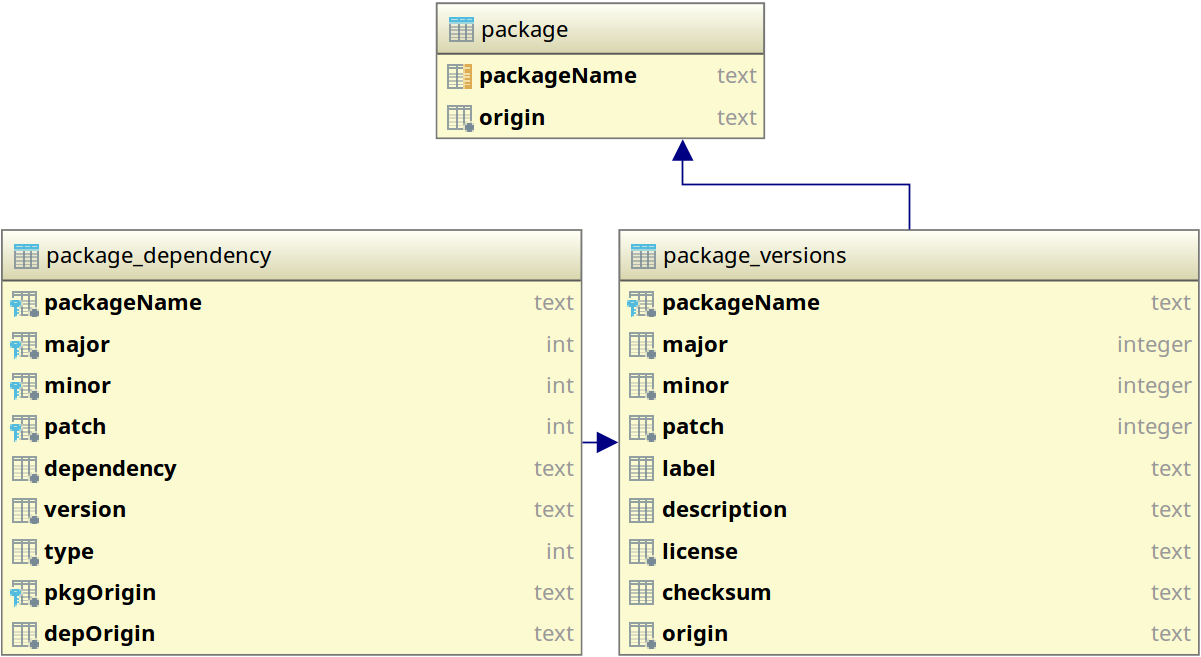
\includegraphics[width=1.0\textwidth]{pictures/regdb.png}
    \caption{The core database model used in the \regdb package}
    \label{fig:registry_database}
\end{figure}

The \txtl{origin} fields which appear in all three tables reference the origin
registry. This is used for handling both cross-registry dependencies, but also
for storing information about packages from different registries. The latter is
useful for cache-like services, which collect information from many different
registries.

Any particular package version also contains a \txtl{checksum} field. This
field can contain any generic checksum which can be serialized as text, that is
the actual checksum algorithm is defined by the client.

The remainder of the fields stored in the database simply mirror the most
important fields of the package manifests. Certain fields from the package
manifests, like the lifetime hooks, are left out of this database model. The
reason for this being lack of interest by clients. The remaining fields, like
name, description, license, are all of interest when it comes to
discoverability of packages.

Table \ref{tab:regdb_operations} shows the operations provided by the \regdb
package. Generally the operations provided by this package for querying
operations operate on a key matching either the \txtl{package} or
\txtl{package_versions} table. Operations that update the tables usually
operate on package manifests (typically provided by the \txtl{packages}
package).

\begin{table}[H]

\begin{longtable}[c]{@{}ll@{}}
\toprule
\begin{minipage}[b]{0.35\columnwidth}\raggedright\strut
Operation
\strut\end{minipage} &
\begin{minipage}[b]{0.59\columnwidth}\raggedright\strut
Description
\strut\end{minipage}\tabularnewline
\midrule
\endhead
\begin{minipage}[t]{0.35\columnwidth}\raggedright\strut
\txtl{query}
\strut\end{minipage} &
\begin{minipage}[t]{0.59\columnwidth}\raggedright\strut
Searches for packages matching a text query
\strut\end{minipage}\tabularnewline
\begin{minipage}[t]{0.35\columnwidth}\raggedright\strut
\txtl{checkIfPackageExists}
\strut\end{minipage} &
\begin{minipage}[t]{0.59\columnwidth}\raggedright\strut
Check if any package exists with name origin
\strut\end{minipage}\tabularnewline
\begin{minipage}[t]{0.35\columnwidth}\raggedright\strut
\txtl{getInfoAboutPackage}
\strut\end{minipage} &
\begin{minipage}[t]{0.59\columnwidth}\raggedright\strut
Lists all versions of a package matching name, origin, and possibly
version
\strut\end{minipage}\tabularnewline
\begin{minipage}[t]{0.35\columnwidth}\raggedright\strut
\txtl{compareWithNewest}
\strut\end{minipage} &
\begin{minipage}[t]{0.59\columnwidth}\raggedright\strut
Checks if a package manifest is newer than what is known by this
registry
\strut\end{minipage}\tabularnewline
\begin{minipage}[t]{0.35\columnwidth}\raggedright\strut
\txtl{insertNewPackage}
\strut\end{minipage} &
\begin{minipage}[t]{0.59\columnwidth}\raggedright\strut
Inserts a new version of a package manifest
\strut\end{minipage}\tabularnewline
\begin{minipage}[t]{0.35\columnwidth}\raggedright\strut
\txtl{createPackage}
\strut\end{minipage} &
\begin{minipage}[t]{0.59\columnwidth}\raggedright\strut
Creates a package with name and origin
\strut\end{minipage}\tabularnewline
\begin{minipage}[t]{0.35\columnwidth}\raggedright\strut
\txtl{getDependencies}
\strut\end{minipage} &
\begin{minipage}[t]{0.59\columnwidth}\raggedright\strut
Returns a list of dependencies for a package (name, origin, version)
\strut\end{minipage}\tabularnewline
\bottomrule
\end{longtable}

\caption{Operations provided by the \regdb package. Operations named changed
slightly for formatting reasons}

\label{tab:regdb_operations}

\end{table}

\section{The JPM Cache}

The \cache of JPM is responsible for downloading packages, and maintaining the
packages in a local cache.

The local cache acts as a database of known packages. This database contains
both the information needed to know about the database, as well as the binary
containing the package data.

The local cache consists of previously downloaded packages, along with a
locally kept database which matches the type that the \registry uses. The
database kept also track the origin \registry, since the \cache will
potentially download from multiple. The key used for this is the location URI
of each \registry. The name cannot be used, since these differ between each
package.

The primary operation that the \cache exposes is the \txtl{installDependency}
operation. This operation will install a dependency directly into a package.
JPM assumes that dependencies are installed under
\txtl{<pkgRoot>/jpm_packages/<depName>}. Having packages stored under a common
folder makes it easy to locate. This is, for example, useful when needing to
filter out the packages. Common places for this would be version control, or
from JPM when publishing a package.

The \cache will first attempt to retrieve the package from its local database,
if not found it will forward the request to the registry. In order to
forward the request, the operation is fed both the registry and
authentication token.

When a new package is received from a \registry, two parts will be returned:
the binary itself, along with the checksum that the \registry believes the
package to have. Checksums are both checked when initially receiving the
package, but also at every install from the cache. This helps prevent initial
corruption and further protects from the cache itself being corrupted. A more
thorough discussion of this feature can be found in Section
\ref{sec:integrity_check}.

The \cache will maintain a \regdb just like the \registry component does. When
new entries are loaded into the \cache, it will updated the \regdb in a similar
fashion. As a result the \cache is technically capable of performing the exact
same responsibilities as the \registry. This could for example allow for fully
offline downloads assuming the data is already loaded into the cache.

%\begin{listing}[H]
%\begin{minted}{text}
%+---------------+   +----------------+
%| packages      |   | checksum       |
%+---------------+   +----------------+
%       ^                    ^
%       |                    |
%       |    +---------------+
%       |    |
%+---------------+   +----------------+
%| cache         |-->| registry       |
%+---------------+   +----------------+
%       |
%       | (local db)
%       v
%+---------------+
%| registry-db   |
%+---------------+
%\end{minted}
%\caption{}
%\label{lst:}
%\end{listing}

\section{Security}
\label{sec:security}

The authorization of JPM is implemented in the \security service. The \security
service provides two different services, which work together to form the
\security service:

\begin{enumerate}

    \item \textbf{An authentication system:} Responsible for proving identity
        of users.

    \item \textbf{An authorization system:} Responsible for deciding which
        users are allowed to do what.

\end{enumerate}

In this section, the client represents a service which uses the \security
services. The system is written to assume that a client \emph{is not} an actual
user. As a result most operations have been written to support various options
which should not be available to actual users. This means that when the
\security service is deployed, care must be taken to ensure that it is not
reachable by any ordinary user. Only the services which use the \security
service should be able to reach it. The services that use the \security
service, will then proxy only the relevant parts along.

\subsection{Authentication}
\label{sec:authentication}

The authentication system has a user based system. Users authenticate
themselves using a password. A group is a collection of users, which have an
associated set of permission. A single user may be part of many groups, it is
from groups that a user gains permission to use parts of the system. We cover
group permissions in Section \ref{sec:authorization}.

The authentication system is build following recommendations from
OWASP\autocite{OWASP1,OWASP2,OWASP3}. In this section the
authentication implementation, and rules surrounding the system are summarized.

\subsubsection*{Username and Password Rules}

The usernames used for the system are unique and case in-sensitive. The
username is required to be between 1 and 64 characters long. All character
types are allowed in usernames. Encoding of the usernames (and passwords) are
deployment dependent, specifically it depends on the protocol and its
configuration.

Passwords are case sensitive. The only limitation put on password is a length
requirement between 5 and 128 characters.

The maximum lengths used for these are mostly to establish reasonable limits.
Accepting an unlimited amount of data can be of concern for both storage and
amount of network traffic. For data that should be presented, i.e. username,
having a maximum is helpful for the design of user interfaces.

\subsubsection*{Storage}

The usernames and passwords are stored in a SQL database. The database itself,
along with its driver is configurable via the configuration system (See
Section \ref{sec:col}). Passwords are hashed with
BCrypt\footnote{BCrypt is a password hashing algorithm which has been used
by OpenBSD and others}\cite{provos1999future}, each individual password has
its own salt. ``Salting'' a password is the act of adding a randomly
generated string to each password. The salt itself isn't secret,
but is instead used to avoid precomputed reverse lookup tables for
the hashes (rainbow tables).

\subsubsection*{Security Concerns}

Limiting number of login attempts within a period is often recommended. This is
done to avoid brute-force attacks. This isn't possible in Jolie, since the
sender isn't available to Jolie user code. This is most likely due to the fact
that no unique sender ID exists, since Jolie can accept messages from various
types of networks.

\subsubsection*{Authentication Process}

We start the discussion of how the authentication process works by looking at
how a client will successfully authenticate itself, this is shown in Figure
\ref{fig:auth_process}.

During the initial request nothing special really happens. The \security
service collaborates with both the \bcrypt service, along with its own
database. The database contains both \txtl{user} objects and \txtl{session}
objects. The \txtl{user} object has already been explained, and simply contains
the username, the hash of the salted password, and the salt itself. The
\txtl{session} object represents an active session. It contains the actual
token, which is a string generated by a cryptographically secure random number
generator. Along with this token, the object contains a timestamp for
generation, and a reference to the user object which created the session. The
timestamp will be used for implementing timeouts for the session.

At the end of the initial request, the client receives the token. This token is
what the client will have to provide for every privileged operation.  An
invalidation of a session may occur. This would ordinarily happen due to a
logout, or potentially a timeout which is handled by the client. The \security
service also supports checking the ``freshness'' of a session token, by making
sure it isn't older than some amount of time. This could be useful for ensuring
re-authentication before critical operations, such as changing your password.

\begin{figure}
    \begin{center}
    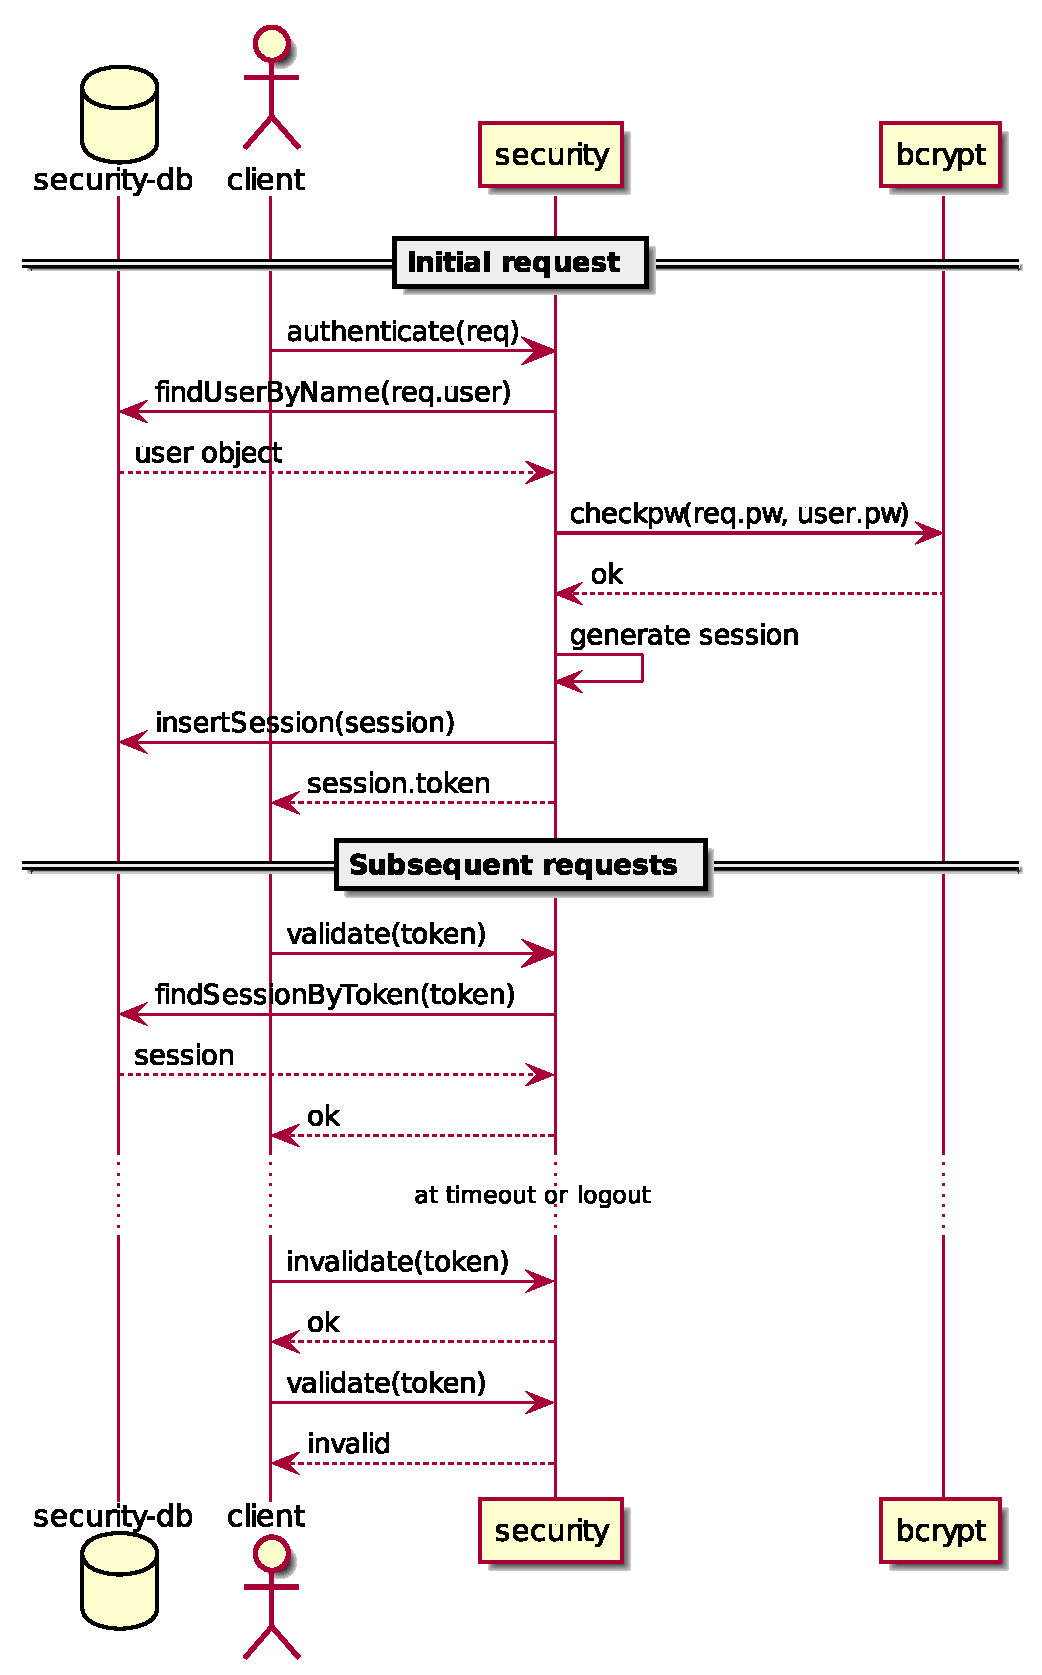
\includegraphics[width=0.8\textwidth]{package_manager/auth_sequence.eps}
    \end{center}
    \caption{The authentication process when successful}
    \label{fig:auth_process}
\end{figure}

Figure \ref{fig:auth_process} showed us the successful case. Internally,
validation will be performed at most steps. In the case of failure at
any of these steps a generic error message will be returned to the
client. The error message will only indicate if it was a user error or a
server error. This way an attacker cannot abuse the error messages for
information. For example given the error message ``Invalid password'' an
attacker would most likely be able to assume that the username itself is
correct.

\subsection{Authorization}
\label{sec:authorization}

The authorization system is based on an ``Access Control
Matrix''\cite{sandhu1994access} to define its security model. An access control
matrix, is a matrix $A$, where $A_{ij}$ contains the \emph{rights} that
\emph{role} $i$ has for \emph{resource} $j$.

A \emph{right} is a single piece of information. It describes something that an
entity is allowed to do for a specific resource in a role. In this
implementation a right is a simple string.

A \emph{resource} represents any entity that can have any rights associated
with it. This could, for example, be a file, which might have associated rights
such as ``read'' and ``write''.

A \emph{role} is some entity which have a set of rights for resources. In the
implementation roles are represented by \emph{groups}. A group is a
collection of users, which are provided by the authentication system.

Table \ref{tab:acm_example} shows an access control matrix for a few files,
which can be either read from or written to.

\begin{table}[H]
  \begin{center}
  \begin{tabular}{ | l | l | l | l | }
    \hline
            & \textbf{File 1}        & \textbf{File 2}      & \textbf{File 3}
    \\ \hline
    \textbf{Group 1} & read, write   & read                 &
    \\ \hline
    \textbf{Group 2} & read          & read                 & read, write
    \\ \hline
  \end{tabular}
  \end{center}

  \caption{A sample access control matrix for some computer files, which can be
      read from and written to by different groups}

  \label{tab:acm_example}
\end{table}

\subsection{Permissions in Registries}

The \registry service is the only consumer of the \security service. On top of
this service the \registry service implements the security model JPM uses. JPM
supports users these map one-to-one with the user model of the \security
service. On top of this JPM supports teams which are supported by a single
underlying group. The purpose of a team is to allow for multiple users to all
have ownership of a single package. Every single user and team get their own
group, user groups only have a single member, while a team group has members
corresponding to the team. The user groups are named \txtl{users.<name>}, and
teams \txtl{groups.<name>}.

When a package is downloaded from or published to the \registry the user's
permissions will be checked. For a user to download a package, the user must be
in a group having the \txtl{read} (or \txtl{write} for publishing) right for
the corresponding resource. Each package has an associated resource called
\txtl{packages.<name>}. A wild card resource (\txtl{packages.*}) also exists.
The wild card resource represents every single package, thus if a group holds
the \txtl{packages.*/read} right then that group is allowed to download ever
package in the \registry. This is exactly how a \registry might provide guest
downloads.

\subsection{Authentication in JPM}

When a user successfully authenticates, the authorization framework will
provide an authentication token proving the user's identity.

For user convenience the JPM system does not require a valid username and
password combination for every privileged operation. To avoid this, JPM will
store the authentication token returned by the \registry. These are stored in a
file on the file-system.

The authentication token is saved instead of the username and password.  Since
if an attacker were to gain access to both the username and password, she would
be able to gain full control over the user, this includes being able to
generate new authentication tokens.

If an attacker instead were to gain only the authentication token, the damage
is not as bad. The attacker would still be able to pose as the user, but only
while the authentication token is valid.

\section{Putting it all Together: Starting Packages}

In this section we will explore what happens when the \txtl{jpm start} command
is invoked. It will cover everything from the front-end all the way to the
registry and back. We won't cover implementation details, as many of the
details are either uninteresting or have been covered elsewhere.

The package we'll be working on is the calculator system, in particular the
starting of the \txtl{calculator} service. We cover how this system is made
into package in Section \ref{sec:calculator_packages}.

From the \txtl{calculator}'s root the user runs:

\begin{minted}{text}
dan@host:/calculator # jpm start
\end{minted}

\subsection{The \txtl{jpm} Binary}

This invokes the \txtl{jpm} binary. This causes the front-end service to be
started with a 

\subsection{The JPM Front-End (\txtl{jpm-cli})}

\subsection{The JPM Back-End (\txtl{jpm})}


TODO I'm not sure we need this.

\section{Examples and Discussion}

\subsection{The Calculator System}

Continuing with the ``modulearized'' version of the calculator system from
Section \ref{sec:module_examples}.

The first step in making these usable from the package manager is of course to
create package manifests. This action becomes fairly straight forward,
especially since we already have a system working with the Jolie module system.
The package manifest for the \txtl{multiplication} package is shown in Listing
\ref{lst:multiplication_package}. The only significant multiplications here are
perhaps a version number, and a formalization of dependencies (in this case the
\txtl{numbers@1.0.0} package).

\begin{listing}[H]
\begin{minted}{json}
{
    "name": "multiplication",
    "description": "An multiplication package",
    "license": "MIT",
    "authors": ["Dan Sebastian Thrane <dathr12@student.sdu.dk>"],
    "main": "main.ol",
    "version": "1.0.0",
    "dependencies": [{ "name": "numbers", "version": "1.0.0" }]
}
\end{minted}
\caption{Package manifest for the \txtl{multiplication} package}
\label{lst:multiplication_package}
\end{listing}

The other package manifests will look fairly similar. The dependency graph ends
up mimicking the system architecture exactly. However there are some subtle
problems associated with the current approach.

Currently the calculator will always download the \txtl{numbers} package,
despite not directly depending on it. This happens due to the dependency on
\txtl{multiplication} which itself depends on \txtl{numbers}. However the
\txtl{calculator} service really only depends on \txtl{numbers} if
\txtl{multiplication} is embedded. At this point this may seem like a minor
detail, but this can get vastly more complicated if there are more dependencies
(which themselves may have dependencies and so on).

The solution to this problem, is to make sure the package manager will only
download the files we actually need, and no more. This would mean if no
embedding is ever performed, we will need only the dependencies required to
perform interfacing. If embedding is required we will need both the interface
dependencies along with a concrete implementation.

For the sake of simplicity the same dependency system is used. It is
recommended that every service separately publishes its interface and concrete
implementation. This approach has the added benefit of allowing multiple
implementations of same service. For closed source services a single package
containing only the interface could be published.

Depending on if an embedding is desired the concrete implementation can simply
be listed as a dependency, the interface dependency will implicitly be picked
up (from the concrete implementation's dependencies). If an embedding is
\emph{never} desired a dependency can be made to just the interface package.

This then begs the question of when to use a concrete implementation over a
dependency. TODO say something.

Additionally JPM might benefit from optional dependencies which are only when
certain conditions are made, for example during some ``development build''.
This might prove to be a decent compromise, allowing for the convenience of
embedding without directly forcing users of the package to also depend on it.

\subsection{Using Lifetime Hooks to Improve Development Workflow}

In this example we will discover how the use of Jolie lifetime hooks can
improve the development workflow. In this example we will look at a hybrid
Jolie-Java service. The service itself will be written in Jolie, using an
internal Java service to perform some of the computational heavy-lifting.  The
\txtl{packages} service, which performs package manifest validation, used in
the package manager is an example of such a package type. The primary flow and
communication is performed entirely by Jolie, while the more ``computationally
heavy'' parts, like parsing, are handled by the internal Java service.  This
architecture is illustrated in Figure \ref{fig:jolie_java_service}.

\begin{listing}[H]
\begin{minted}{text}
+----------------------------------------+
|                                        |
| jolie-service ---------+               |
|                        | local         |
|                        | communication |
|                        |               |
|                        v               |
|                      +----------------+|
|                      | java-service   ||
|                      +----------------+|
+----------------------------------------+
\end{minted}
\caption{A Jolie service using an internal Java service}
\label{fig:jolie_java_service}
\end{listing}

The Java service uses Gradle as its build system. The build system is capable
of producing a JAR file. The Jolie engine requires this file to be included in
the classpath in order to perform the embedding. If the file is placed in the
\txtl{lib} directory this will happen automatically.

A small bash script was made to run JAR creation through Gradle, and then copy
the artifact into the \txtl{lib} directory. Interested readers may find both
the Gradle build script and bash script in Appendix 3. Both scripts are
relatively simple, but should be a sufficient starting point.

The file structure of the project is shown in Listing
\ref{lst:java_jolie_file_structure}. The \txtl{build} file is the script which
performs the entire build and copies it into the \txtl{lib} directory.

\begin{listing}[H]
\begin{minted}{text}
.
|-- build
|-- java-service
|   |-- build.gradle
|   `-- src/main/java/dk/thrane/jolie/JavaService.java
|-- main.ol
`-- package.json
\end{minted}
\caption{}
\label{lst:java_jolie_file_structure}
\end{listing}

Assuming a lot of changes are made to the Java service, this would mean two
commands would almost always be required to create a new iteration of the
build. This can be minimized by creating a \txtl{pre-start} hook as shown in
Listing \ref{lst:pre_start_hook}. Having it as a part package manifest makes
the intent very clear. Having some home-made build script would instead rely
entirely on convention. Such conventions may vary from project to project,
while having it as a part of the package manifest would remain consistent
across all JPM packages.

\begin{listing}[H]
\begin{minted}{json}
"events": { "pre-start": "./build" }
\end{minted}
\caption{A \txtl{pre-start} hook for performing compilation of the internal
    Java-service}
\label{lst:pre_start_hook}
\end{listing}

The JPM lifetime hooks aim to enforce the implicit workflow a project typically
has by making it explicit.

TODO Testing...



\chapter{Conclusion}
\label{cha:conclusion}
In this thesis, we have presented two new extensions to the Jolie programming
language, namely, the module system and the configuration system.

The module system allows the Jolie engine to think about collections of files
which are rooted in a particular directory. This introduced the new module
include primitive.

The configuration system is built upon the module system to allow configuration
of modules. The configuration system introduced the new configuration format
(COL) which allows the user configuration of modules. COL files entirely
replace the old way of doing configuration, through ordinary Jolie source
files. COL files present a way of configuring a module, in a similar syntax to
that of ordinary Jolie code.

Input ports and output ports, the primitives used by Jolie for communication,
can be configured. The configuration of ports, follow the features that
the Jolie language already provided. As a result, it is now possible to
move freely between externally bound output ports to embedding the same
service, entirely from the configuration. This was previously not possible
without changing the source code of a service.

Parameters allow for configuration values to be provided to a service.
Parameters are automatically type-checked at deployment time of a service. Due
to constraints within the Jolie engine, a new verification stage was added to
the Jolie engine.

The configuration system introduced a notion of interface parametricity through
interface rebinding. This feature allows developers to write generic Jolie
services which use the, already existing, aggregation feature. This was also
not previously doable without changing the source code of the service.

We also presented the Jolie Package Manager (JPM). JPM manages a new concept of
packages. Packages are an extension of the Jolie modules, also developed in
this thesis. Package extends modules, by adding a package manifest which
describes the package.

Packages can be published to a registry. Published packages are downloaded from
the registry, by the JPM tool, and installed into packages.  The JPM tool also
provides a variety of features that include registry account management,
lifetime hooks, and integrity checking of packages.



\appendix
\chapter{Appendix}
\section{Appendix A: JPM Manifest Specification}\label{package-specification}

This document covers the specification of the file which defines a
package. The format used for this document will be JSON, but the format
and whether or not to allow for several documents is still up for
discussion. For now we should avoid using any features which the generic
Jolie value cannot support.

\subsection{Purpose}\label{purpose}

The purpose of the package document is to define what a package is.
Every Jolie package will contain such a document, and it describes
several important properties about the package. These properties are
described in the section ``Format and Properties''.

\subsection{Table of Contents}\label{table-of-contents}

\begin{itemize}
\tightlist
\item
  \protect\hyperlink{format-and-properties}{Format and Properties}

  \begin{itemize}
  \tightlist
  \item
    \protect\hyperlink{name}{name}
  \item
    \protect\hyperlink{version}{version}
  \item
    \protect\hyperlink{license}{license}
  \item
    \protect\hyperlink{authors}{authors}
  \item
    \protect\hyperlink{private}{private}
  \item
    \protect\hyperlink{main}{main}
  \item
    \protect\hyperlink{dependencies}{dependencies}
  \item
    \protect\hyperlink{dependency}{dependency}

    \begin{itemize}
    \tightlist
    \item
      \protect\hyperlink{name-1}{name}
    \item
      \protect\hyperlink{version-1}{version}
    \item
      \protect\hyperlink{registry}{registry}
    \end{itemize}
  \item
    \protect\hyperlink{registries}{registries}
  \item
    \protect\hyperlink{registry-1}{registry}

    \begin{itemize}
    \tightlist
    \item
      \protect\hyperlink{name-2}{name}
    \item
      \protect\hyperlink{location}{location}
    \end{itemize}
  \end{itemize}
\end{itemize}

\hypertarget{format-and-properties}{\subsection{Format and
Properties}\label{format-and-properties}}

\hypertarget{name}{\subsubsection{name}\label{name}}

\textbf{Name:} \texttt{name}

\textbf{Optional:} false

\textbf{Type:} \texttt{string}

\textbf{Description:} The \texttt{name} property uniquely defines a
package in a registry. Every registry must only contain a single package
with a given name.

\textbf{Rules:}

\begin{itemize}
\tightlist
\item
  The name of a package is \emph{not} case-sensitive
\item
  The length of a name is less than 255 characters
\item
  Names are US-ASCII
\item
  Names may only contain unreserved URI characters (see section 2.3 of
  \href{https://www.ietf.org/rfc/rfc3986.txt}{RFC 3986})
\end{itemize}

If any of these rules are broken the JPM tool should complain when
\emph{any} command is invoked. Similarly a registry should reject any
such package.

\hypertarget{version}{\subsubsection{version}\label{version}}

\textbf{Name:} \texttt{version}

\textbf{Optional:} false

\textbf{Type:} \texttt{string}

\textbf{Description:} This property describes the current version of
this package.

\textbf{Rules:}

\begin{itemize}
\tightlist
\item
  The version string must be a valid SemVer 2.0.0 string (see
  http://semver.org/spec/v2.0.0.html)
\end{itemize}

\hypertarget{license}{\subsubsection{license}\label{license}}

\textbf{Name:} \texttt{property\_name}

\textbf{Optional:} false

\textbf{Type:} \texttt{string}

\textbf{Description:} Describes the license that this package is under.

\textbf{Rules:}

\begin{itemize}
\tightlist
\item
  Must be a valid identifier. See https://spdx.org/licenses/
\end{itemize}

\hypertarget{authors}{\subsubsection{authors}\label{authors}}

\textbf{Name:} \texttt{authors}

\textbf{Optional:} false

\textbf{Type:}
\texttt{string\textbar{}array\textless{}string\textgreater{}}

\textbf{Description:} Describes the authors of this package

\textbf{Rules:}

\begin{itemize}
\tightlist
\item
  The array must contain at least a single entry
\item
  Each entry should follow this grammar:
\end{itemize}

\begin{verbatim}
name ["<" email ">"] ["(" homepage ")"]
\end{verbatim}

\hypertarget{private}{\subsubsection{private}\label{private}}

\textbf{Name:} \texttt{private}

\textbf{Optional:} true

\textbf{Type:} \texttt{boolean}

\textbf{Description:} Describes if this package should be considered
private. If a package is private it cannot be published to the
``public'' repository.

\textbf{Rules:}

\begin{itemize}
\tightlist
\item
  By default this property has the value of \texttt{true} to avoid
  accidential publishing of private packages.
\end{itemize}

\hypertarget{main}{\subsubsection{main}\label{main}}

\textbf{Name:} \texttt{main}

\textbf{Optional:} true

\textbf{Type:} \texttt{string}

\textbf{Description:} Describes the main file of a package.

\textbf{Rules:}

\begin{itemize}
\tightlist
\item
  The value is considered to be a relative file path from the package
  root.
\end{itemize}

\hypertarget{dependencies}{\subsubsection{dependencies}\label{dependencies}}

\textbf{Name:} \texttt{dependencies}

\textbf{Optional:} true

\textbf{Type:} \texttt{array\textless{}dependency\textgreater{}}

\textbf{Description:} Contains an array of dependencies. See the
``dependency'' sub-section for more details.

\textbf{Rules:}

\begin{itemize}
\tightlist
\item
  If the property is not listed, a default value of an empty array
  should be used
\end{itemize}

\hypertarget{dependency}{\subsubsection{dependency}\label{dependency}}

\textbf{Type:} \texttt{object}

\textbf{Description:} A dependency describes a single dependency of a
package. This points to a package at a specific point on a specific
registry.

\hypertarget{name-1}{\paragraph{name}\label{name-1}}

\textbf{Name:} \texttt{name}

\textbf{Optional:} false

\textbf{Type:} \texttt{string}

\textbf{Description:} Describes the name of the dependency. This refers
to the package name, as defined earlier.

\textbf{Rules:} A dependency name follows the exact same rules as a
package name.

\hypertarget{version-1}{\paragraph{version}\label{version-1}}

\textbf{Name:} \texttt{version}

\textbf{Optional:} false

\textbf{Type:} \texttt{string}

\textbf{Description:} Describes the version to use

\textbf{Rules:}

\begin{itemize}
\tightlist
\item
  Must be a valid SemVer 2.0.0 string
\item
  (This property follows the same rules as the package version does)
\end{itemize}

\hypertarget{registry}{\paragraph{registry}\label{registry}}

\textbf{Name:} \texttt{registry}

\textbf{Optional:} true

\textbf{Type:} \texttt{string}

\textbf{Description:} This describes the exact registry to use. If no
registry is listed the ``public'' registry will be used.

\textbf{Rules:}

\begin{itemize}
\tightlist
\item
  The value of this property must be a valid registry as listed in the
  \texttt{registries} property.
\end{itemize}

\hypertarget{registries}{\subsubsection{registries}\label{registries}}

\textbf{Name:} \texttt{registries}

\textbf{Optional:} true

\textbf{Type:} \texttt{array\textless{}registry\textgreater{}}

\textbf{Description:} Contains an array of known registries. See the
registry sub-section for more details.

\textbf{Rules:}

\begin{itemize}
\tightlist
\item
  This property contains an implicit entry which points to the public
  registry. This registry is named ``public''.
\end{itemize}

\hypertarget{registry-1}{\subsubsection{registry}\label{registry-1}}

\textbf{Type:} \texttt{object}

\textbf{Description:} A registry describes a single JPM registry. A JPM
registry is where the package manager can locate a package, and also
request a specific version of a package.

\hypertarget{name-2}{\paragraph{name}\label{name-2}}

\textbf{Name:} \texttt{name}

\textbf{Optional:} false

\textbf{Type:} \texttt{string}

\textbf{Description:} This property uniquely identifies the registry.

\textbf{Rules:}

\begin{itemize}
\tightlist
\item
  A name cannot be longer than 1024 characters
\item
  The name cannot be ``public''
\item
  No two registries may have the same name
\end{itemize}

\textbf{TODO:}

\begin{itemize}
\tightlist
\item
  Encoding of name
\item
  Should the length limit be dropped? There is no technical reason for
  the limit
\end{itemize}

\hypertarget{location}{\paragraph{location}\label{location}}

\textbf{Name:} \texttt{location}

\textbf{Optional:} false

\textbf{Type:} \texttt{string}

\textbf{Description:} Describes the location of the registry.

\textbf{Rules:}

\begin{itemize}
\tightlist
\item
  Must be a valid Jolie location string (e.g.
  ``socket://localhost:8080'')
\end{itemize}



\printbibliography
\end{document}
